% Created 2021-10-31 Sun 22:27
% Intended LaTeX compiler: pdflatex
\documentclass[phd,black, hidelinks]{PrincetonThesis}
\usepackage[utf8]{inputenc}
\usepackage[T1]{fontenc}
\usepackage{graphicx}
\usepackage{grffile}
\usepackage{longtable}
\usepackage{wrapfig}
\usepackage{rotating}
\usepackage[normalem]{ulem}
\usepackage{amsmath}
\usepackage{textcomp}
\usepackage{amssymb}
\usepackage{capt-of}
\usepackage{hyperref}
\usepackage{minted}
\usepackage{tabularx}
\usepackage{epsfig}
\usepackage{times}
\usepackage{hyperref}
\usepackage{graphicx}
\usepackage{mathtools}
\usepackage{pbox}
\usepackage{lscape}
\usepackage{multirow}
\usepackage{hhline}
\usepackage{array}
\usepackage[toc,page]{appendix}
\usepackage{framed}
\usepackage{float}
\usepackage{pgfplots}
\usepackage{amsmath}
\DeclareMathOperator*{\argmin}{arg\,min}
\DeclareMathOperator*{\argmax}{arg\,max}
\newcommand{\compconj}[1]{\overline{#1}}
\newcommand{\euler}{e}
\usepackage{dsfont}
\usepackage{bm}
\usepackage{natbib}
\newcommand{\tablespace}{\vspace{.3\baselineskip}}
\newcolumntype{C}[1]{>{\centering}m{#1}}
\newcolumntype{P}[1]{>{\centering\arraybackslash}p{#1}}
\title{Time series: Defining a search engine}
\advisor{Dr. Ioannis Katakis}
\department{Computer Science}
\degreemonth{February}
\degreeyear{2022}
\author{Philipp Beer}
\date{\today}
\title{Time Series: Defining a Search Engine}
\hypersetup{
 pdfauthor={Philipp Beer},
 pdftitle={Time Series: Defining a Search Engine},
 pdfkeywords={},
 pdfsubject={},
 pdfcreator={Emacs 27.2 (Org mode 9.4.6)}, 
 pdflang={English}}
\begin{document}

\pgfplotsset{compat=1.17}
\begin{frontmatter}
\begin{thesisabstract}
This is abstract.
\end{thesisabstract}
\begin{acknowledgements}
These are the acknowledgements.
\end{acknowledgements}
\end{frontmatter}
\cleardoublepage
\chapter{Abstract}
\label{sec:orgf3abe26}
\chapter{Purpose}
\label{sec:org9f7d761}
The purpose of this thesis is to explore the possibility of creating a time series series search engine.

ts forecasting big challenge, stats approaches, ML approaches which lag - however, little explored area how curated datasets can improve forecasting results and possibly improve of data analytics results or just simply see which time series show similar properties. lots of work similarity measures but compute intensivenes forbids large scale use of them when large data amounts are present

explore a method here that provides value insight on similarity is flexible and computationally significantly cheaper than what is represents the current standard

\chapter{Introduction}
\label{sec:org6adfd4d}
Time series is often described as "anything that is observed sequentially over time" which usually are observed at regular intervals of time \cite{hyndman2014forecasting}. They can be described as collection of observations that are considered together in chronological order rather than as individual values or a multiset of values. Their representation can be described as ordered pairs:
\(S = (s_1,s_2,\dots,s_n)\) where \(s_n = (t_n,v_n)\). \(t_n\) can be a date, timestamp or any other element that defines order. \(v_1\) represents the observation at that position in the time series.

Time series are utilized to analyze and gain insight from historic events/patterns with respect to the observational variable(s) and their interactions. A second area of application is forecasting. Here time series are utilized to predict the observations that occur in future under the assumption that the historic information can provide insight into the behavior of the observed variables.

\citeauthor{Fu_2011} in their work \cite{Fu_2011} categorized time series research into (1) representation, (2) indexing, (3) similarity measure, (4) segmentation, (5) visualization and (6) mining. Research in these different fields started taking off in the second half of the 20\textsuperscript{th} century. For example in \cite{_str_m_1969} the authors worked on questions of representation via sampling the sampling of time series in \citeyear{_str_m_1969}. All these different research areas always have to deal with the challenges that inhibit time series data. Generally datasets in this domain are large. Through this time series data incorporates the similar obstacles as high dimensional data, namely the "curse of dimensionality" \cite{Tang_2019} and requiring large computational efforts in order to generate insights. And as will be discussed in \ref{org7eca1e7} there are applications fields where vast amounts of time series are generated and a comparison between them is required.

In this thesis we will focus on creating a algorithm allowing the fast and meaningful comparison of an input time series or template against a vast array time series. Within the research many different areas and approaches have been attempted (at list here). However, there is a tendency to apply the simplest methods possible to achieve the desired results. For time series those are mainly Euclidean Distance and Dynamic Time Warping. While those methods will be explored in section \ref{org8eba293} it can be said that those methods are simple, easy to understand and produce mostly reliable results in their respective application domains. Good performance is not their strong suit. Therefore, our approach is targeted to achieving comparable capability in identifying similar series, while achieving it with a significant reduction in computational complexity.

\section{Applications}
\label{sec:org7c3cf06}
\label{org7eca1e7}
Time series are encountered everywhere. Any metric that is captured over time can utilized as time series. Granularity can be used as descriptor for the sampling rate of a series or more general how often measurements for a particular metric are taken. This granularity has a tendency to increase as well. As example consumer electronics that capture health and fitness data can mentioned. Or sensors which are utilized in the automotive industry or heavy machinery where they are employed to capture information for predictive maintenance applications.\\

In the financial industry time series are a very fundamental component of decision making, like the development of stock prices over time or financial metrics of interest. The same is true for macro economic information or metrics concerning social structures in society, etc.\\

In the medical field time series are also ubiquitous. Whether they relate to patient date like blood pressure. The bio statistics field utilizes electro-graphical data like electrocardiography, electroencephalography and many others. In more aggregate medical analysis like toxicology analysis of drug treatments for vaccine approvals they are utilized and in many forms of risk management, for example, population level obesity levels.\\

In engineering fields the utilization is often times similar to the above but it also require that information that is captured in time series is transferred between locations in an efficient manner. For example voice calls are required to be transferred between the participants in a fast manner and with minimized levels of noise in the data. Another interesting industrial example in the biomedical technology field is Neuralink which aims to implement a brain-machine-interface (BMI) utilizing mobile hardware like smartphones as the basis for its computation. Here a large of amount of time series data is generated which requires quick processing to generate real-time information. \citeauthor{Musk_2019} describes a recording system with 3072 electrodes generating time series data \cite{Musk_2019} that is used to capture the brain information and visualized in real-time \cite{Siegle_2017}.

Time series data is paramount to a wide variety of areas, relating to many different fields. Looking at the trajectory it seems likely that going forward more time series data on a higher granularity will be generated. This in turn increases the need to be able process, analyze, compare and respond to the data with methods that are faster than today's standard options.


\section{Organization of this thesis}
\label{sec:org85cb8e7}
The rest of this thesis is organized as follows:

\section{{\bfseries\sffamily TODO} to be integrated}
\label{sec:org57c5b76}
\begin{itemize}
\item refer to previous work on measures of similarity and outcome
\item measure of similarity required
\item challenges with time series (domains, granularity, length, outliers)
\item area of signal processing interesting methods
\end{itemize}
\chapter{Related work}
\label{sec:org28f0674}
\label{org8eba293}
Related work addressing the idea of time series search engine focuses on the system architecture and the data processing and pipelining aspect of this such an architecture \cite{Zhang_2012}. However, in \citeyear{Keogh_2000} \citeauthor{Keogh_2000} also applied a dimensionality reduction technique (Piecewise Constant Approximation) to execute fast search similarity search in  large time series databases. Other papers address domain specific questions like the introduction of a "Time-series Subimage Search Engine for archived astronomical data" \cite{Kang_2021}.

In order to be able to describe the closeness of time series or multiple time series to each a measure for similarity is required. In the literature various general measures and corresponding computation methods can be found. \citeauthor{Wang_2012} reviewed time series measures and categorized the similarity measures into 4 categories: (1) lock-step measures, (2) elastic measures, (3) threshold-based measures, and (4) pattern-based measures. \citeauthor{Zhang_2020} classify similarity measures in the categories: (1) time-rigid methods (Euclidean Distance), (2) time-flexible measures (dynamic time-warping), (3) feature-based measures (Fourier coefficients), and (4) model-based methods (auto-regression and moving average model) \cite{Zhang_2020}. Lock-step measures include the L\textsubscript{p}-norms (Manhattan and Euclidean Distance) as well as Dissimilarity Measure (DISSIM). Elastic measures include metrics like Dynamic Time Warping (DTW) and edit distance based measures like Longest Common Subsequence (LCSS), Edit Sequence on Real Sequence (EDR), Swale and Edit Distance with Real Penalty. An example for threshold-based measures are threshold query based similarity search (TQuEST). And Spatial Assembling Distance (SpADe) is an example for pattern-based measures. In another paper, \citeauthor{Gharghabi_2020} classify the space of similarity measures by the the most common measures into: (1) Euclidean Distance, (2) Dynamic Time Warping (DTW), (3) Least Common Subsequence (LCSS), and (4) K-Shape.

Dynamic Time Warping (DTW) is an elastic measure, meaning that it is flexible in its comparision of points. This is in opposition to Euclidean Distance (ED) where each point is compared with its counterpart on the time series of comparision. DTW has been introduced by \citeauthor{Berndt94usingdynamic} in \citeyear{Berndt94usingdynamic} and its key advantage is the fact that comparison is applied on a one-to-many-basis allowing the comparison of regions from one series to regions of the other time series. This gives it the capability to warp peaks or valleys between different time steps of the two series as the resulting distance metric. As will be shown in section \ref{org50fa20e} this comes at the price of time complexity which renders it effectively useless in practice when applied to large scale data sets.

Other attempts are also made in introducing new distance metrics. \citeauthor{Gharghabi_2020} introduced a new metric called MPdist (Matrix Profile Distance) which is more robust than Euclidean Distance (ED) - more details can be found in section \ref{org1b35bfe} - and Dynamic Time Warping (DTW) - more details can be found in section \ref{org50fa20e} - and computationally preferable. Interestingly, due to the use of subsequences in the comparison of two time series its time complexity ranges from \(\mathcal{O}(n^2)\) in the worst case, to \(\mathcal{O}(n)\) in the best case and with this can provide a significant advantage of prevalent methods like ED or DTW.

The other research area of interest for our task is time series representation. It concerns itself with the optimal combination of reduction of the data dimensionality but adequate capture of its particular properties. With these methods feats like minimizing noise, managing outliers can be achieved. For many activities this is also the basis for the reduction of time complexity in the resulting algorithms that analyze and compare the time series.

According to \citeauthor{Li_2019} the following methods are common methods for this task: (1) Discrete Fourier Transformation (DFT), (2) Singular Value Decomposition (SVD), (3) Discrete Wavelet Transformation (DWT), (4) Piecewise Aggregate Approximation (PAA), (5) Adaptive Piecewise Constant Approximation (APCA), (6) Chebyshev polynomials (CHEB), (7) Symbolic Aggregate approXimation, and others \cite{Li_2019}. In their paper, \citeauthor{Pang_Liu_Peng_Peng_2018} mention (1) Singular Value Decomposition (SVD), (2) Frequency-Domain transformation, (3) Piecewise Linear Representation (PLR), (4) model-based method, and (5) symbolic representation.

\section{Dimensionality Reduction related to Singular Value Decomposition}
\label{sec:orge4891ed}
Singular Value Decomposition is a fundamental matrix factorization technique with a plethora of applications and use cases. It's value comes from the capability of generating low rank approximations of data matrices that allow to represent the matrix values via the unitary matrices \(\bm{U} \in \mathbb{C}^{n \times n}\) and \(\bm{V} \in \mathbb{C}^{m \times m}\). The columns in in \(\bm{U}\) and  \(\bm{V}\) are orthonormal. The remaining matrix \(\bm{\Sigma} \in \mathbb{R}^{n \times m}\), is a diagonal matrix with non-negative entries.

The power of the SVD is its ability to provide a low-dimensional approximation to high-dimensional data \cite{brunton2019data}. High dimensional data is often determined by a few dominant patterns which can be described by a low-dimensional attractor. Therefore, a prime application for the SVD is dimensionality reduction. It is complementary to the Fast Fourier Transform (FFT) which lays at the core of this work. \citeauthor{brunton2019data} describe it as the generalization of the FFT.

Principal Component Analysis (PCA) is a very common application of the SVD. It was developed by \citeauthor{Pearson01} in \citeyear{Pearson01}. The main idea of PCA is to apply the SVD to a dataset centered around zero and subsequently computing the covariance of the centered dataset. Through the computation of the eigenvalues and their identifying the largest values the most important principal components are identified. Those are responsible for the largest variance in the dataset. And similar to the SVD their ranking and subsequent filtering can be used to focus on the most important components that allow to recreate majority of the of the variance in the dataset.

The Fast Fourier Transform (FFT) is based upon the Fourier Transform introduced by Joseph Fourier in early 19\textsuperscript{th} century to analyze and analytically represent heat transfer in solid objects \cite{fourier1822theorie}. This transform is a fundamental component of modern computing and science in general. It has transformed how technology can be used in the in 20\textsuperscript{th} century in areas such as image and audio compression and transfer. The concept will be introduced in more detail in section \ref{orgb49bdde}. Its core idea is to represent the data to be transformed as the coefficients of a basis of sine and cosine eigenfunctions. It is similar to the principles of the SVD with the notable difference that the basis are an infinite sum of sine and cosine functions. The ability to reduce to the transformed data to few key components is the same as in SVD and PCA.

\section{Symbolic Aggregate approXimation}
\label{sec:orga085728}
A dimensionality reduction technique that does not built on SVD and is geared directly towards time series is the Symbolic Aggregate approXimation (SAX) algorithm. Its core idea is to transform a time series into a set of strings via piecewise aggegrate approximation (PAA) and a conversion of the results via a lookup table \cite{Lin_2003}. Starting with PAA the reduction of a time series \(T\) of length \(n\) in vector \(\bar{S} = \bar{s_1}, \bar{s_2}, \dots, \bar{s_w}\) of length \(w\) where \(w < n\), can be achieved through the following computation:
\begin{equation}
\bar{s_i} = \frac{w}{n} \sum_{j=\frac{n}{w}(i-1)+1}^{\frac{n}{w}i} s_j
\end{equation}

\begin{figure}[htbp]
\centering
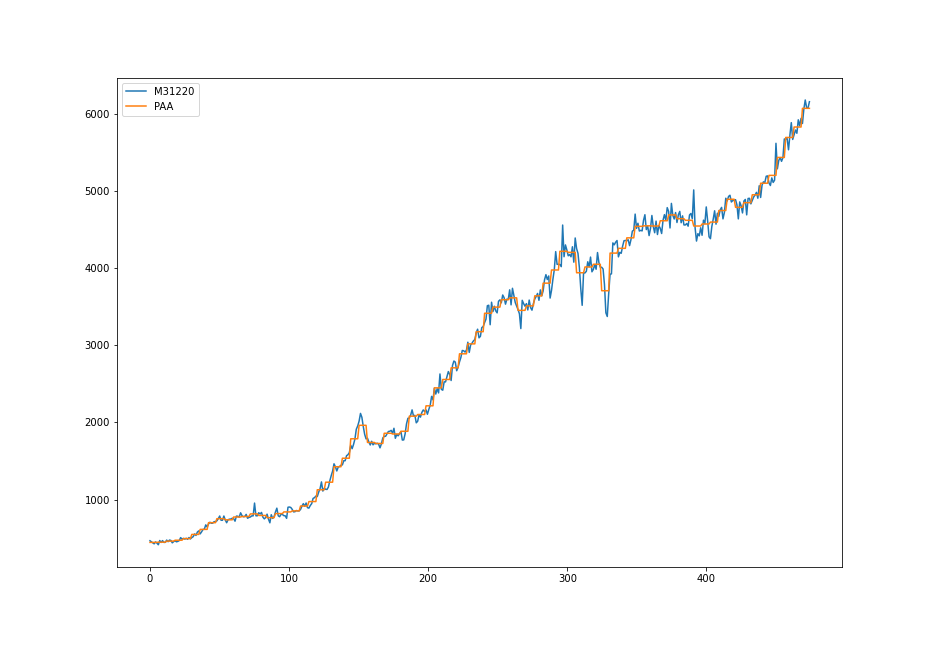
\includegraphics[width=.9\linewidth]{./img/paa_example.png}
\caption{\label{fig:org2685122}Piecewise Aggregate Approximation - M4 example: M31220 (window size - 6)}
\end{figure}

This simply computes the mean of each of sub sequences determined through parameter \(w\). An example from the M4 dataset can be seen in figure \ref{fig:org2685122}. For its application in SAX the time series are standardized or mean normalized, so that the comparison happens on the same amplitude. From this representation the data is further transformed to obtain a discrete representation via the mapping of the values computated via PAA to a symbolic representation of a letter. The used discretization should accomplish equiprobability in the assignments of the symbols \cite{Lin_2007}. The authors show by example of taking subsequences of length 128 from 8 different time series that the resulting PAA transformation has a Gaussian dstribution. This property does not hold for all series. And in place where it does not hold the algorithm performance deteriorates. If the assumption that the data distribution is Gaussian is true, breakpoints that will produce equal-sized areas can be obtained from a statistical table. The breakpoints are defined as \(B = \beta_1, \beta_2, \dots, \beta_{a-1}\) so that the area under a Gaussian curve \(N(0,1)\) from \(\beta\)\textsubscript{i} to \(\beta_{i+1}= \frac{1}{a}\)  (\(\beta\)\textsubscript{0} and \(\beta\)\textsubscript{a} are defined as -\(\inf\) and \(\inf\)) \cite{Lin_2007}. Table \ref{tab:org48e1903} shows the value ranges for values of a from 3 to 10 and has been reproduced from \cite{Lin_2007}.

\begin{table}[htbp]
\caption{\label{tab:org48e1903}Lookup table - reproduced from \citeauthor{Lin_2007}}
\centering
\begin{tabular}{lrrrrrrrr}
\(\beta\)\textsubscript{i} & 3 & 4 & 5 & 6 & 7 & 8 & 9 & 10\\
\hline
\(\beta\)\textsubscript{1} & -0.43 & -0.67 & -0.84 & -0.97 & -1.07 & -1.15 & -1.22 & -1.29\\
\(\beta\)\textsubscript{2} & 0.43 & 0 & -0.25 & -0.43 & -0.57 & -0.67 & -0.76 & -0.84\\
\(\beta\)\textsubscript{3} &  & 0.67 & 0.25 & 0 & -0.18 & -0.32 & -0.43 & -0.52\\
\(\beta\)\textsubscript{4} &  &  & 0.84 & 0.43 & 0.18 & 0 & -0.14 & -0.25\\
\(\beta\)\textsubscript{5} &  &  &  & 0.97 & 0.57 & 0.32 & 0.14 & 0\\
\(\beta\)\textsubscript{6} &  &  &  &  & 1.07 & 0.67 & 0.43 & 0.25\\
\(\beta\)\textsubscript{7} &  &  &  &  &  & 1.15 & 0.76 & 0.52\\
\(\beta\)\textsubscript{8} &  &  &  &  &  &  & 1.22 & 0.84\\
\(\beta\)\textsubscript{9} &  &  &  &  &  &  &  & 1.28\\
\hline
\end{tabular}
\end{table}

Based into which \(\beta\) category a value of PAA fits a symbol is assigned. "\textbf{a}" is reserved for values smaller than \(\beta\)\textsubscript{1} and values execeeding \(\beta\)\textsubscript{a-1} is assigned the last symbolic value which differs depending on how many categories are chosen.

As stated before, this method relies on the fact that the data is normally distributed. Therefore, it can be great to detect for example anomalies in streaming data. Also the distance computation is preserved on the PAA values. However, the distance computation is still based on Euclidean Distance (ED) and has the same time complexity as before, but for fewer data points compared to the original series.
\chapter{Underlying Concepts}
\label{sec:org15899a6}
This section gives an overview of the concepts utilized in this thesis to generate the baseline performance of the algorithm against which our

\section{Euclidean Distance}
\label{sec:org6b71cad}
\label{org1b35bfe}
Euclidean Distance is the most widely used distance metric in the research of time series. It is either used as a metric on its on or a as metric used used inside other methods to compute distances, for example, computation of distance of subsections of the data (\cite{Faloutsos_1994}) or to compute the distance between various points of two time series (see section \ref{org50fa20e}). Having two time  series \(S = \{s_1, s_2, \dots, s_n\}\) and \(Q = \{q_1, q_2, \dots, q_n \}\) both of length \(n\) the Euclidean distance can be computed as:
\begin{equation}
D(S,Q) = \sqrt{\sum_{i=1}^{n}{(S_i,Q_i)^2}}
\end{equation}

It is a measure that is easy to compute and comprehend and gives intuitive input for the distance of two time series. From the standpoint of time complexity the algorithm is applicable also to larger datasets with \(\mathcal{O}(n)\). Its simplicity also creates some limitations. For example, to compute the euclidean distance between two series their length needs to be the same. Furthermore, it can be easily impacted in its results by the presence of outliers or increased levels of noise. It is not elastic with respect to the warping of information between two series in which effects that could indicate similarity happen even at slightly disparate steps. 

Despite its shortcomings it is a prominent metric and widely used for distance calculations for short comings. Some of its limitations are addressed by more sophisticated metrics that utilize its computation as component.

\section{Dynamic Time Warping}
\label{sec:org6e72811}
\label{org50fa20e}
\citeauthor{Berndt94usingdynamic} introduced Dynamic Time Warping in \citeyear{Berndt94usingdynamic} finding the minimal alignment between two time series computed through a cost matrix and identifying the minimized path through the matrix starting from the final elements of each time series. This warps the points in time between the different series as shown in figure \ref{fig:orgcbebb14}.

\begin{figure}[htbp]
\centering
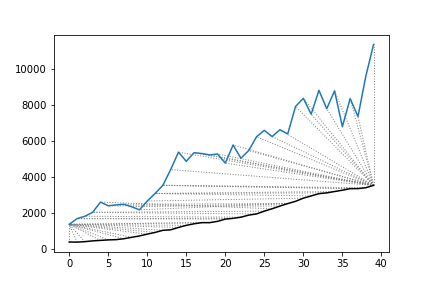
\includegraphics[width=.9\linewidth]{./img/dtw_ex_plain.png}
\caption{\label{fig:orgcbebb14}Dynamic Time Warping - M4 Example: Y5683 and Y5376}
\end{figure}

Two series \(S = \{s_1, s_2, \dots, s_n\}\) of length \(n\) and \(Q = \{q_1, q_2, \dots, q_m\}\) of length \(m\) are considered. For the series a n-by-m cost matrix \(M\) is constructed. Each element in the matrix represents the respective i\textsuperscript{th} and j\textsuperscript{th} element of each of the two series which contains the distance of those to points:
\begin{equation}
m_{ij} = D(s_i, q_j)
\end{equation}

where often time euclidean distance is used as distance function \(D(s_i, q_j) = (s_i - q_j)^2\). From the matrix a warping path \(P\) is chosen, \(P = p_1,p_2,\dots, p_k, \dots, p_K\) where:

\begin{equation}
\max(m,n) \leq k < m+n-1
\end{equation}

The warping path is constrained with bound with the following condition \(p_1 = (1,1)\) and \(p_K = (m,n)\). That means that both first elements of each series, as well as, the last element of each series are bound to each other in the computation. The warping path also is continuous. This means that from each chosen element \(p_k\) only the neighboring elements to the left, right and diagonally can be chosen for the continuation of the path: \(p_k= (a,b)\) and \(p_{k-1} = (a',b')\) with \(a-a' <=1\) and \(b-b' <= 1\). The path elements \(p_k\) are also monotonous, meaning that \(a-a' \geq 0\) and \(b-b' \geq 0\). From the resulting matrix considering the mentioned constraints a cumulative distance \(\gamma(i,j)\) is computed recursively:
\begin{equation}
\gamma(i,j) = D(s_i,q_j) + \min \{\gamma(i-1, j-1), \gamma(i-1, j), \gamma(i, j-1)\}
\end{equation}
Therefore, the path can obtained by the following definition:
\begin{equation}
DTW(S,Q) = \min_{P: Warping Path}\left\{\sum_{k=1}^K \sqrt{p_k}\right\}
\end{equation}

Figure \ref{fig:org232cb5e} provides an example for a warping path result.

\begin{figure}[htbp]
\centering
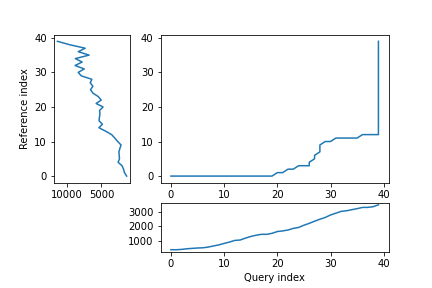
\includegraphics[width=.9\linewidth]{./img/dtw_3way.png}
\caption{\label{fig:org232cb5e}Warping path example - M4 data: Y5683 and Y5376}
\end{figure}

The challenge with the application of DTW is the time complexity of the algorithm \(\mathcal{O}(m*n)\) due to the fact that the distance compuation needs to be executed for each element of each series. Various methods for speed improvements have been introduced. The favorite principle was described by \citeauthor{Ratanamahatana_2004}. They introduced an adjustment window condition that where it is assumed that the optimal path does not drift very far from the diagonal of the cost matrix \cite{Ratanamahatana_2004}. However, this does not change the fundamental nature of the algorithm and computing DTW for multiple time series against a database of time series will require days of computation time even on modern computer architectures. 

In favor of DTW needs to be stated, that it is flexible with regards to the series used. The compared time series do not require to have the same length and can still be compared. This is a property that is not avaiable with Euclidean Distance. However, the user also needs to be aware of outliers in either data set which can lead to a clustering of the warping path or pathological matches around those extreme points in the series. 

Therefore in practice, Dynamic Time Warping is not a method suitable for comparing a single time series against a large array of series when speed is an important criterion as well as the handling of outliers in the dataset.

\begin{enumerate}
\item Similarity through decomposition
\label{sec:orgd8d461f}
\begin{itemize}
\item introduce time series decomposition (reference in \cite{hyndman2014forecasting})
\item trend and seasonality (mention assumptions about period)
\end{itemize}
\end{enumerate}
\section{Fast Fourier Transform}
\label{sec:org960db2f}
\label{orgb49bdde}
In Fourier analysis the Fast Fourier Transform (FFT) is a more efficient implementation of the Discrete Fourier Transform (DFT) that utilizes specific properties. The Discrete Fourier transform is based on the Fourier Transform (FT) which concerns itself with the representation of functions which in turn is built upon the Fourier series. We will give a brief introduction to them. However, a thorough introduction can be found in \cite{brunton2019data}. The principal idea Fourier analysis follows is that it can project functions - i.e. Fourier Transform - and data vectors - i.e. Discrete Fourier Transform - into a coordinate system defined by orthogonal functions (sine and cosine). To get the exact representation of a function or a data vector it has be done in infinitely many dimensions.
\subsection{Inner Product of Functions and their norms}
\label{sec:org4ae6f6f}
To get to the properties of of data under the Fourier transform we must start with the Hermitian inner product (\cite{ratcliffe2006foundations}) of functions in Hilbert spaces, \(f(x)\) and \(g(x)\) (\(\compconj{g}\) denotes the complex conjugate of \(g\)) in the domain \(x \in [a,b]\):
\begin{equation}
\langle f(x),g(x) \rangle = \int_a^b f(x) \, \compconj{g}(x)dx
\end{equation}
This means that the inner product of the functions \(f(x)\) and \(g(x)\) are equivalent to the integral between \(a\) and \(b\). This notion can be transferred to the vectors generated by these functions under discretization. We want to show that under the limit of data values \(n\) of the functions \(f(x)\) and \(g(x)\) approaching infinity, \(n \to \infty\) the inner product of the vectors approach the inner product of the functions. We take \(\vec{f} = [f_1, f_2, \dots, f_n]^T\) and \(\vec{g}= [g_1, g_2, \dots, g_n]^T\) and define the inner product as:
\begin{equation}
\langle\vec{f},\vec{g}\,\rangle = \sum_{k=1}^n f(x_k) \, \compconj{g}(x_k).
\end{equation}
This formula behaves as desired but grows in its value as more and more data points are added, meaning more data points correspond to higher values, which hinders comparison of series with shorter length. So a normalization is added to counter the effect. The normalization occurs through the domain chosen for the analysis \(\Delta x = \frac{b-a}{n-1}\):
\begin{equation}
\frac{b-a}{n-1} \langle\vec{f},\vec{g}\, \rangle =\sum_{k=1}^n f(x_k) \, \vec{g}(x_k)\Delta x.
\end{equation}
This corresponds to the Riemann approximation of continuous functions \cite{anton1998calculus}. As more data more data points are collected and therefore \(n \to \infty\) the inner product converges to the inner product of the underlying functions.

The norm of the inner product of the functions can also be expressed as integral:
\begin{equation}
\|f\|_2 = (\langle f,\, f\rangle)^{\frac{1}{2}} = \sqrt{\langle f, \, f \rangle} = \left( \int_a^b f(x) \, \compconj{f}(x)dx  \right)^{\frac{1}{2}}.
\end{equation}
The last required step is transferring the applicability from a finite-dimensional vector space to an infinite-dimensional vector space. For this we can use the Lebesgue integrable functions or square integrable functions \(L^2([a,b])\). All functions with a bounded norm define the set of square-integrable functions \cite{brunton2019data}. Next we will show how a Fourier series is a projection of a function onto the orthogonal set of sine and cosine functions.

\subsection{Fourier Series}
\label{sec:org4fe6529}
As the name suggests the Fourier series is an infinite sum of sine and cosine functions of increasing frequency. The mapped function is assumed to be periodic. A simple case of \$2\(\pi\)\$-periodic can be shown as:
\begin{equation}
f(x) = \frac{a_0}{2} + \sum_{k=1}^\infty (a_k \cos(kx) + b_k\sin(kx)).
\end{equation}
If one imagines that this transformation projects the function onto a basis of cosine and sine, \(a_k\) and \(b_k\) are coefficients that represent the coordinates of where in that space the function is projected.
\begin{equation}
a_0 = \frac{1}{\pi} \int_{-\pi}^{\pi} f(x)dx
\end{equation}
\begin{equation}
a_k=\frac{1}{\pi} \int_{-\pi}^{\pi} f(x) \cos(kx)dx
\end{equation}
\begin{equation}
b_k=\frac{1}{\pi} \int_{-\pi}^{\pi} f(x) \sin(kx)dx.
\end{equation}
Those coefficients are are acquired through integration and multiplication of sine and cosine.
This expression can be re-written in the form of an inner product:
\begin{equation}
a_k = \frac{1}{\|\cos(kx)\|^2} \langle f(x),\, \cos(x)\rangle
\end{equation}
\begin{equation}
b_k = \frac{1}{\|\sin(kx)\|^2} \langle f(x),\, \sin(x)\rangle
\end{equation}
The squared norms are \(\|\cos(kx)\|^2 = \|\sin(kx)\|^2 = \pi\). However, this only works for 2\(\pi\)-periodic functions. For real world data this is obviously most often not the case. Therefore, another term needs to be added that stretches the 2\(\pi\)-periodicity to length of the observed domain \([0,L)\) with \(\frac{kx}{L}*2\pi\). This L-periodic function is then given by:
\begin{equation}
f(x) = \frac{a_0}{2} + \sum \left( a_k\cos \left( \frac{2\pi kx}{L} \right) + b_k \sin \left( \frac{2\pi kx}{L}  \right)  \right)
\end{equation}
This modifies the integrals for the coefficients to:
\begin{equation}
a_k = \frac{2}{L} \int_{0}{L} f(x) \cos \left( \frac{2\pi kx}{L}  \right)
\end{equation}
\begin{equation}
b_k = \frac{2}{L} \int_{0}{L} f(x) \sin \left( \frac{2\pi kx}{L}  \right)
\end{equation}
One can write the formula utilizing Euler's formula
\begin{equation}
\euler^{ikx} = \cos(kx) + i \sin(kx),
\end{equation}
utilizing complex coefficients (\(c_k = \alpha_k + i \beta_k\)):
\begin{equation}
\begin{aligned}
 f(x)={} & \sum_{k=- \infty}^{\infty} c_k \euler^{ikx} = \sum_{k=-\infty}^{\infty} (\alpha_k + i \beta_k) (\cos(kx) + i \sin(kx)) \\
 ={} & (\alpha_0 + i \beta_0) + \sum_{k=1}^{\infty} \left[ (a_{-k} + a_k) \cos(kx) + (\beta_{-k} - \beta_k) \sin(kx) \right] + \\
 & i \sum_{k=1}^{\infty} \left[ (\beta_{-k} + \beta_{k}) \cos(kx) - (\alpha_{-k}  - \alpha_k) \sin(kx)  \right].
\end{aligned}
\end{equation}
For real-valued functions it needs to be ensured that \(c_{-k} = \compconj{c}_k\) through \(\alpha_{-k}= \alpha_k\) and \(\beta_{-k}= - \beta_k\). It also needs to be shown that theb basis provided by sine and cosine are orthogonal. This is only the case if both functions have the same frequency. We define \(\psi_k = \euler^{ikx}\) for \(k \in \mathcal{Z}\). This means that our sine and cosine functions can only take integer values as frequencies. To show that those are orthogonal over the interval \([0,2\pi)\) we look at the following inner product and equivalent integral:

\begin{equation}
\langle \psi_j,\,\psi_k \rangle = \int_{-\pi}^{\pi} \euler^{jkx} \euler^{-ikx}dx =
\begin{dcases}
\mathrm{if} \, j \neq k & \int_{-\pi}^{\pi} \euler^{i0x} =  2\pi \\
\mathrm{if} \, j = k & \int_{-\pi}^{\pi} \euler^{i(j-k)x} =  0 \\
\end{dcases}
\end{equation}
When \(j = k\) the integral reduces to 1, leaving \(2\pi\) as the result of the interval to be integrated. In cas \(j \neq k\) the expansion of the Euler's formula expression cancels out the cosine values and sine evaluated integer multiples of \(\pi\) is equal to \(0\). Another way to express the inner product is via the Kronecker delta function:
\begin{equation}
\langle \psi_j, \psi_k \rangle = 2\pi \delta_{jk}.
\end{equation}
This result can be transferred to a non-2\(\pi\)-periodic basis \(e^{i2\pi \frac{kx}{L}}\) in \(L^2 ([0,L))\). And the final step in the Fourier series is to show that any function f(x) is a projection on the infinitie orthognal-vector space  space that is spanned by cosine and sine functions:
\begin{equation}
f(x) = \sum_{k=-\infty}^{\infty} c_k \psi_k(x) = \frac{1}{2\pi} \sum_{k=-\infty}^{\infty} \langle f(x),\,\psi_k(x)\rangle\psi_k(x).
\end{equation}
The factor \(1/2\pi\) normalizes the projection by \(\|\psi_k\|^2\).

\subsection{Fourier Transform}
\label{sec:orga7d59b8}
So far, the Fourier series can only be applied to periodic functions. This means that after the length of the interval the function repeats itself. With the Fourier transform an integral is defined in which the domain goes to infinity in the limit such that functions can be defined without repeating itself. So if we define a Fourier series and its coefficients as:
\begin{equation}
\begin{aligned}
f(x)={} & \frac{a_0}{2} + \sum_{k=1}^{\infty} \left[ a_k \cos\left( \frac{k\pi x}{L} \right) + b_k \sin \left( \frac{k\pi x}{L} \right)  \right] \\
= & \sum_{k=-\infty}^{\infty} c_k \euler^{\frac{ik\pi x}{L}}
\end{aligned}
\end{equation}
\begin{equation}
c_k = \frac{1}{2L} \langle f(x), \, \psi_k \rangle = \frac{1}{2L} \int_{-L}^{L} f(x)\euler^{- \frac{ik\pi x}{L}}dx.
\end{equation}
Our frequencies are defined by the \(\omega_k = k\pi/L\). By taking a limit as \(L \to \infty\) two properties are achieved:
\begin{enumerate}
\item the frequencies become a continuous range of frequencies
\item a infinite precision in the representation of our time series in the Fourier space is achieved.
\end{enumerate}
We define \(\omega_k = k\pi/L\) and \(\Delta \omega_k = \pi /L\). As \(L \to \infty\), \(\Delta \omega \to 0\). We take the take the complex coefficient \(c_k\) in its integral representation and apply the limit to \(L\):
\begin{equation}
f(x) = \lim_{\Delta \omega \to 0} \sum_{k=-\infty}^{\infty} \frac{\Delta \omega}{2\pi} \int_{-\frac{\pi}{\Delta \omega}}^{\frac{\pi}{\Delta \omega}} f(\xi)\euler^{-ik\Delta \omega \xi}d \xi \, e^{ik \Delta \omega x}.
\end{equation}
By taking the limit the inner product of the coefficient, i.e. the integral with respect to \(\xi\) turns into the Fourier transform of \(f(x)\) and the first part of the Fourier transform pair written as \(\hat{f}\) and defined as, \(\hat{f} \triangleq \mathcal{F}(f(x))\):
\begin{equation}
\hat{f}(\omega) = \mathcal{F}(f(x)) = \int_{-\infty}^{\infty} f(x)\euler^{-i\omega x}dx
\end{equation}
The inverse Fourier transform utilizes \(\hat{f}(\omega)\) to recover the original function \(f(x)\):
\begin{equation}
f(x) = \mathcal{F}^{-1}(\hat{f}(\omega)) = \frac{1}{2\pi} \int_{-\infty}^{\infty} \hat{f}(\omega)\euler^{i\omega x}d\omega.
\end{equation}
As long as \(f(x)\) and \(\hat{f}(\omega)\) belong to the Lebesgue integrable functions the integrals converge. In effect this means that functions have to tend to 0 as \(L\) goes to infinity.
\subsection{Discrete Fourier Transform}
\label{sec:org34de652}

In order to be able to apply the Fourier transform to time series a they need to be applicable to discrete data as well. The Discrete Fourier Transform (DFT) approximates the Fourier transform on discrete data \(\textbf{f} = [f_1, f_2, \dots, f_n]^T\) where \(f_j\) is regularly spaced.
The discrete Fourier transform pair is defined as:
\begin{equation}
\hat{f}_k = \sum_{j=0}^{n-1} f_j\euler^{-2\pi jk/n},
\end{equation}
\begin{equation}
f_k = \frac{1}{n} \sum_{j=0}^{n-1}\hat{f}_j\euler^{i2\pi jk/n}.
\end{equation}
Via the DFT \(\textbf{f}\) is mapped into the frequency domain \(\hat{\textbf{f}}\). As before the output in the resulting DFT matrix is complex valued, meaning that it can be (and is) heavily used for physical interpretations for example in engineering questions as well.
\subsection{Fast Fourier Transform}
\label{sec:org63fe976}

So far we have shown that the Fourier Series and the Discrete Fourier Transform can provide an exact representation of any arbitrary function or data generating process without requiring any assumptions or parameter settings. In the time complexity however we are dealing with an implementation that has complexity \(\mathcal{O}(n^2)\). As an example, let's consider the M4 dataset, which will be introduced in section \ref{org44d15b1}. The longest series has \(n=9919\) datapoints. Given the time complexity of the DFT this will include \(\mathcal{O}(n^2)=9919^2=9.8 \times 10^8\) or about 1 billion operations. With the Fast Fourier Transform this can be reduced to a time complexity of \(\mathcal{O}(n \log(n))\). In our example this results to \(\mathcal{O}(9919 \log(9919)) = 1.3 \times 10^5\) or roughly 130,000 thousand operations. This is a improvement of factor 7,538. It is also an indication that when to time series it still provides very fast computation times.

To be able to convert the DFT to the FFT a multiple of 2 datapoints is required. For example, take \(n=2^6=64\). In this case the DFT matrix can be written as follows:
\begin{equation}
\hat{\textbf{f}} = \textbf{F}_{64}\textbf{f} =
\begin{bmatrix}
\textbf{I}_{32} & -\textbf{D}_{32} \\
\textbf{I}_{32} & -\textbf{D}_{32} \\
\end{bmatrix}
\begin{bmatrix}
\textbf{F}_{32} & \textbf{0} \\
\textbf{0} & \textbf{F}_{32} \\
\end{bmatrix}
\begin{bmatrix}
\textbf{f}_{\text{even}} \\
\textbf{f}_{\text{odd}}
\end{bmatrix},
\end{equation}
where \(\textbf{I}_{32}\) is the Identity matrix. \(\textbf{f}_{\text{even}}\) contain the even index elements of \(\textbf{f}\), i.e. \(\textbf{f}_{\text{even}} = [f_0, f_2,f_4, \dots, f_n]\) and \(\textbf{f}_{\text{odd}}= [f_1,f_3,f_5, \dots, f_{n-1}]\). This process is executed recursively. In our example it would continue like this: \(\textbf{F}_{32} \to \textbf{F}_{16} \to \textbf{F}_{8} \to \dots\) This is done down to \(\textbf{F}_2\) where the resulting computations are excuted on \(2 \times 2\) matrices, which is much more efficient than the DFT computations. Of course, it always has be broken down with the same process of taking the even and odd index rows of the resulting vectors. This significantly reduces the required computations to \(\mathcal{O}= (n \log(n))\). Important is also that if a series does not have the length \(n\) of a multiple of two, it is expedient to just pad the vector with zeros up to the length of the next power of two.
\subsection{Parseval's Theorem}
\label{sec:org40a344c}
\label{org8d4ed6b}
One property that the Fourier Transform has is central to the approach in this work. It is called Parseval's Theorem. It states that the integral of square of a function is equal to the integral of the square of its transform. In other words, the \$L\textsubscript{2}\$-norm is preserved. This can be expressed as:
\begin{equation}
\int_{-\infty}^{\infty} \lvert \hat{f}(\omega) \rvert^2 d\omega = 2\pi \int_{-\infty}^{\infty} \lvert f(x) \rvert^2 dx.
\end{equation}

This property is important to us for multiple reasons. It tells us that angles and lengths are preserved in the frequency domain. This means, the different time series are comparable in the frequency domain they way they are in the time domain. And a second consequence that can be derived from this property is that frequencies with comparatively little power in the power spectrum (see section \ref{org41bae4d}) can be removed from the representation in the frequency domain and still allow very similar reconstruction of the original time series. We will use this property in only comparing the top n most energetic frequencies of the all the frequencies computed in the Fourier transform (see section \ref{org9f9de98}).
\subsection{Power Spectrum}
\label{sec:orge5d94e0}
\label{org41bae4d}
One important property of time series transformed is the resulting power spectrum or power spectral density (PSD). This concept comes from the signal processing field. The power spectrum denoted as \(S_{xx}\) of a time series \(f(t)\) describes the from which frequencies a signal is composed. It describes how the power of a sinusoidal signal is distributed over frequency. Even in the case of non-physical processes it is customary to describe it as power spectrum or the energy of a frequency per unit of time \cite{press1992numerical}.

To obtain the power spectrum we are converting our input vector via the FFT:
\begin{equation}
\begin{bmatrix}
f_0 \\
f_1 \\
\vdots \\
f_n \\
\end{bmatrix}
\xrightarrow{FFT}
\begin{bmatrix}
\hat{f}_0 \\
\hat{f}_1 \\
\vdots \\
\hat{f}_n \\
\end{bmatrix}
\end{equation}
The resulting vector contains the complex values obtained through the FFT. We define the complex value contained in arbitrary value of the vector:
\begin{equation}
\hat{f}_j \triangleq \lambda
\end{equation}
The complex value is represented as \(\lambda = a + ib\). We compute the power of the particular frequency:
\begin{equation}
\hat{f}_j = \lVert\lambda \rVert^2= \lambda \compconj{\lambda} = (a + ib)(a - ib) = a^2 + b^2.
\end{equation}
This is the magnitude of the particular frequency. In figure \ref{fig:orgd27be2d} an exemplartory time series from the M4 dataset (see section \ref{org44d15b1}) is visualized alongside the corresponding power spectrum of its Fourier Transform. The x-axis represents the corresponding frequencies obtained by the FFT, while the y-axis indidicates the energy contained in the respective frequencies. The x-axis is plotted in log-scale. An important property is the fact that the frequencies in the power spectrum differ depending on the length of the of the time series. A frequency of \(k_a=2\) in a series \(S_1\) length \(n_{S_1}=5\) is equivalent to a frequency \(k_b=4\) in a series \(S_2\) of length \(n_{S_2}= 10\).
\begin{figure}[htbp]
\centering
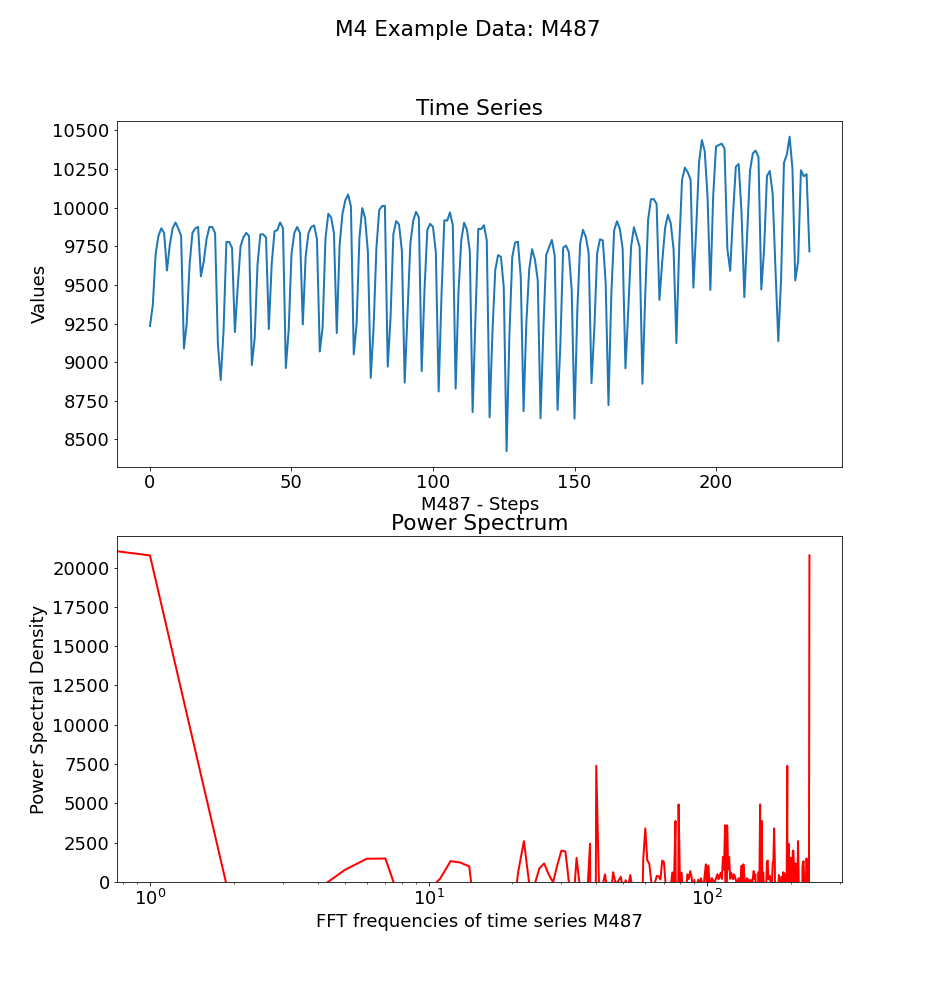
\includegraphics[width=.9\linewidth]{./img/fft_example.png}
\caption{\label{fig:orgd27be2d}Power Spectrum M4 - Example: M487}
\end{figure}
\subsection{Spectral Leakage}
\label{sec:orge38faf1}
\label{orgeb5c515}
The Fast Fourier Transform (FFT) assumes that the signal continues infinitely in time and that there no discontinuities. However, any signal in the real world, including time series has finite data points. If the time domain is an integer multiple of of the frequency \(k\) than each records connects smoothly to the next. Real world processes generally do not follow sinusoidal wave forms and can contain significant amounts of noise, as well as phase changes and trends. So if the signal is not an integer multiple of the sampling frequency \(k\) this signal leaks into the adjacent frequency bins. See figure \ref{fig:orgd27be2d} in the power spectrum plot around 10\textsuperscript{1}. Both on the left a likely example of spectral leakage can be observed. As we intend to use the ranked by energy leve frequencies to look for similarities between time series this can be an issue as we want to avoid that the leaked frequencies are utilized for the determination of the most important frequencies. We will look at window functions to address this issue.
\subsection{Window Functions}
\label{sec:org58bf7ae}
In the field of signal processing a lot of research has been conducted to combat the spectral leakage described in section \ref{orgeb5c515}. One way of addressing spectral leakage are window functions, also called tapering or apodization functions. They help reduce the undesired effects of spectral leakgage. They have been used successfully in various areas of signal processing, like speech processing, digital filter design and spectrum estimation \cite{kumar2011}. Spectrum estimation is the field we will apply them here.

The windows applied to data signals affect several properties of harmonic processors like the Fast Fourier Transform (FFT), like detectability, resolution, and others \cite{harris1978}. The window functions are designed such that in the spectral analysis they help reduce the side lobes next to the main beams of the spectral output of the Fast Fourier Transform (FFT). A side effect is that the main lobe broadens and thus the resolution is decreased \cite{kumar2011}. The sprectral power in a particular bin contains leakage from neighboring bins. The window function brings the data  down to zero at the edges of the time series. An example applied to a series from the M4 dataset can be seen in figure \ref{fig:org9fc523e}.

\begin{figure}[htbp]
\centering
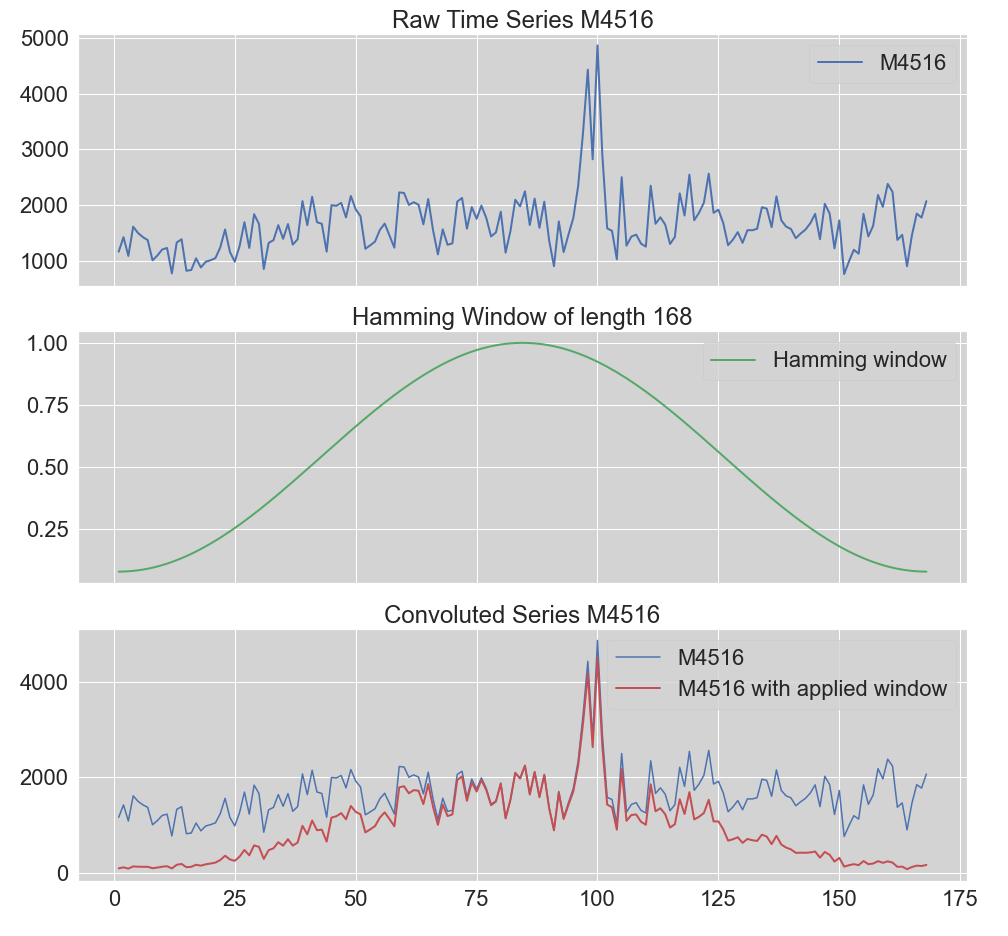
\includegraphics[width=.9\linewidth]{./img/ham_window_example.png}
\caption{\label{fig:org9fc523e}Hamming window example with M4 time series M4516}
\end{figure}


The Hamming window is named after R.W. Hamming. It is one of many window functions and is defined as
\begin{equation}
w(n) = 0.54 - 0.46 \cos \left( \frac{2\pi n}{M - 1}  \right) \quad
0 \leq n \leq M - 1,
\end{equation}
with \(M\) being the length of time series to be covered. As can be seen in the figure, it minimizes the sidelobes created by the FFT, but it also minimizes valid signal at the edge of the time series data.

\subsection{Bartlett's and Welch's Method}
\label{sec:org8c2ba65}
Another approach to address spectral leakage is to average periodograms generated over multiple subsets of the time series. Welch's method is based on Bartlett's method which is described in the following \cite{bartlett1948}. Let us denote the x\textsuperscript{th} periodgram or power spectrum as \(\hat{P}\).
The idea that the average of the computed periodograms is unbiased:
\begin{equation}
\lim_{N \to \infty} E\{\hat{P}_{per}(\euler^{j\omega})\} = P_x(\euler^{j\omega})
\end{equation}
So a consistent estimate of the mean, is a consistent estimate of the power spectrum. If we can assume that the realizations in the time series data are uncorrelated then they result in a consistent estimate of its mean. This means that the variance of the sample mean reduces with the number of measurements. They are inversly proportional. Therefore, averaging periodograms produces a the correct periodogram of the data. If we let \(x_i(n)\) for \(i = 1,2, \dots, K\) be \(K\) uncorrelated realizations of a random process \(x(n)\) over the interval of length \(L\) with \$ 0 \(\le\) n < L\$ and with \(\hat{P}_{per}^{(i)}(\euler^{j\omega})\) the periodogram \(x_i(n)\) is:
\begin{equation}
\hat{P}_{per}^{(i)}(\euler^{j\omega})= \frac{1}{L} \left\lvert \sum_{n=0}^{L-1} x_i(n)\euler^{-jn\omega}  \right\lvert^2 \quad ; \quad
i= 1,2, \dots, K
\end{equation}
These periodograms can then be averaged
\begin{equation}
\hat{P}_x (\euler^{j\omega}) = \frac{1}{K} \sum_{i=1}^K \hat{P}_{per}^{(i)}(\euler^{j\omega})
\end{equation}
and gives us an asymptotically unbiased estimate of the power spectrum. Because of the assumption that the values are uncorrelated, the variance is inversely proportional to the number of measurements K
\begin{equation}
\text{Var} \left\{ \hat{P}_x(\euler^{j\omega})  \right\}= \frac{1}{K} \text{Var}\left\{ \hat{P}_{per}^{(i)}(e^{j\omega}) \right\} \approx \frac{1}{K}P_x^2(\euler^{j\omega})
\end{equation}
However, the assumption that the time series data is uncorrelated does not hold. Bartlett proposed to circumvent that to partition the data into \(K\) non-overlapping sequences of length \(L\) with a time series \(X = \{x_1,x_2,\dots,x_n\}\) of length \(N\) such that, \(N = K \times L\).
\begin{equation}
\begin{aligned}
x_i(n) = x(n + iL) \quad n = & 0,1,\dots,L-1 \\
                         i = & 0,1,\dots,K-1
\end{aligned}
\end{equation}
In consequence, Bartlett's method can be written as:
\begin{equation}
\hat{P}_B(e^{j\omega}) = \frac{1}{N} \sum_{i=0}^{K-1} \left\lvert \sum_{n=0}^{L-1} x(n + iL)e^{-j\omega} \right\rvert^2
\end{equation}
An example of the split of time series can be seen in figure \ref{fig:org3630361}.
\begin{figure}[htbp]
\centering
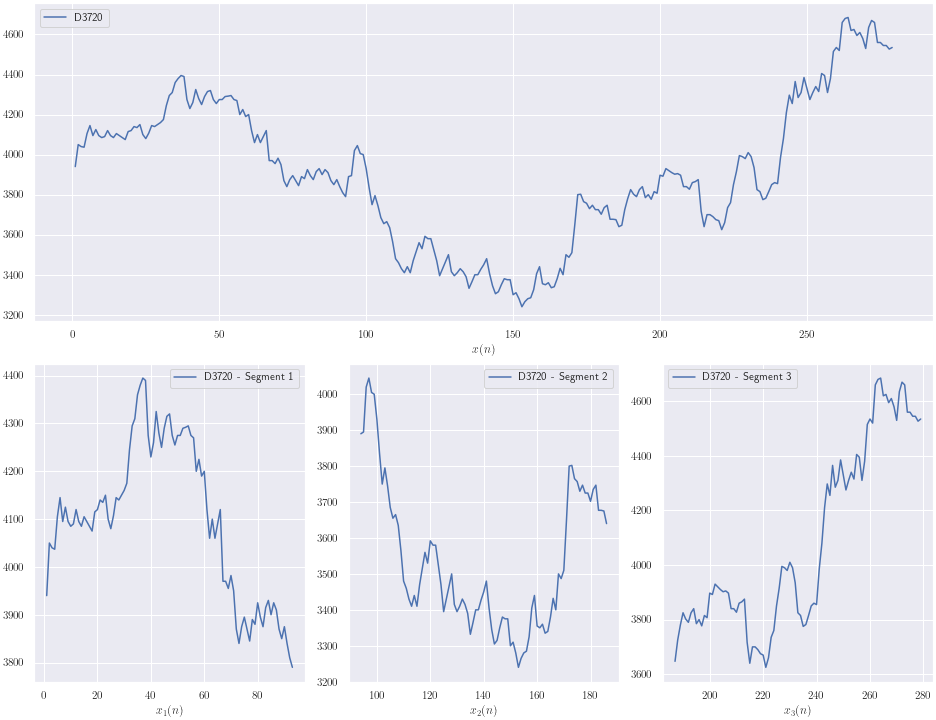
\includegraphics[width=.9\linewidth]{./img/bartlett_example.png}
\caption{\label{fig:org3630361}Bartlett's window example from M4: D3720}
\end{figure}


Welch's method differs in how the windows are applied to the dataset. For Welch's method the windows are not adjacent are overlapping. The original data set is still split into \(K\) sequences of length \(L\) overlapping by \(D\) points with \(0 \leq D < 1\). If the overlapping is defined to be 0, then this method is equivalent to Bartlett's method. An overlap of 50\% can be achieved via \(D = K/2\). The overlapping of the data segments effectively cures the fact that an applied window minimizes the data at the edges of the window. The i\textsuperscript{th} sequence can be described by \(x_i(n)= x(n+iD) \; ; \; n=0,1,\dots,L-1\) with \(L\) being the length of a sequence. \(N\) can be computed by \(N = L + D(K-1)\) where \(K\) is the number of sequences. Welch's method is described by
\begin{equation}
\hat{P}_W(\euler^{j\omega})=\frac{1}{KLU} \sum_{i=0}^{K-1} \left\lvert \sum_{n=0}^{L-1} w(n)x(n+iD)\euler^{-jn\omega}  \right\rvert^2
\end{equation}
with
\begin{equation}
U = \frac{1}{L} \sum_{n=0}^{L-1} \lvert w(n) \rvert^2
\end{equation}
An example of time series split via Welch's method with \(K=4\) can be seen in figure \ref{fig:org60ed02d}.
[[./img/welch\textsubscript{example.png}]
\chapter{Methodology}
\label{sec:org6c5eea8}
\label{orge0400ec}
\section{General Overview}
\label{sec:orge6162e4}
The main idea of our method is to define the underlying frequencies as their most important property to identify similar time series. In a second step additional statistical metrics are used to reduce the number of similar series such that the user of the application can decide which for metrics the comparison should be executed.

The whole process consists of two general phases with further subdivisions of which only the second should be considered for computing the run-time of this method. Phase I is a  prepartory step required to set up the pool of time series which serve as the database from which the closest matches are identified. Phase I consists of:
\begin{enumerate}
\item Data Transformation (see section \ref{orge0cee10})
\item Statistical Metrics Computation (see section \ref{orgfc6d82a})
\end{enumerate}

Phase II describes how a single series considered as template series is matched against all available series in the database (see section \ref{orgc5ae61a}).

\subsection{Data Transformation}
\label{sec:org748bb69}
\label{orge0cee10}
The preparation of the time series pool is done by executing the data transformation for all time series and computing the statistical metrics for all time series (section \ref{orgfc6d82a}). The data transformation is based on the Fast Fourier transform (FFT) and is executed multiple times for each series with multiple transformation types: (1) FFT with original data, (2) FFT with applied Hamming window on each time series, and (3) FFT with Welch's method and a Hamming window applied on each sub series for each time series. For a shorthand in the following "FFT" or "regular FFT" is used to describe the Fast Fourier transform without modification to the original data, "Hamming" is used to describe the FFT with a Hamming window applied to the original data, and "Welch" is used to describe the Fast Fourier transformation while applying Welch's method with a Hamming window on each subseries. The results from all three transformations are kept separately for later comparison to the template series.

After the transformations have been created only the top K (in our case top 5) frequencies, meaning the 5 frequencies with the highest magnitude in the frequency domain are retained and frequency range intervals are created (see section \ref{org9f9de98}). The top K frequencies are then associated with their respective frequency interval (see section \ref{org772d555}). This process is depicted visually in figure \ref{fig:org6a49405}.

\begin{figure}[htbp]
\centering
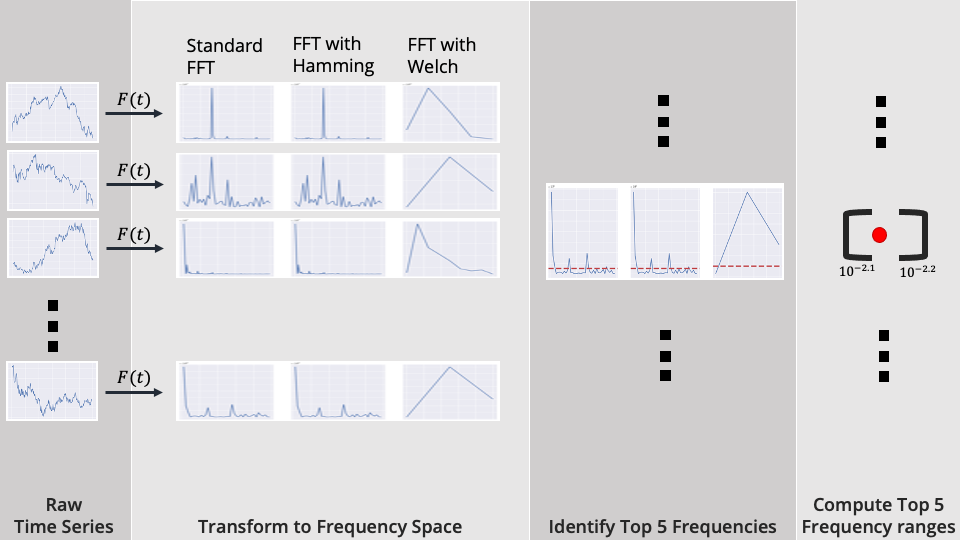
\includegraphics[width=.9\linewidth]{./img/process_fft.png}
\caption{\label{fig:org6a49405}Phase 1a: convert time series pool to frequency space and identify top 5 frequency ranges}
\end{figure}

With the completion of this step we have each time series associated with a list of K frequency intervals orded from lowest magnitude to highest magnitude associated with the respective series. So each time series is described by 5 data points irrespective of the length of the original series. Aside from other benefits this already hints at the fact that comparing 5 datapoints per comparison will be executed significantly faster than comparing hundreds or thousands of data points.

\subsection{Statistical metrics computation}
\label{sec:org840d451}
\label{orgfc6d82a}
Describing a time series only by the top K frequency intervals in the Fourier domain is not sufficient to adequately describe the properties of a time series for matching it with other series. This, in part, is due to the fact that the magnitude of the particular frequency is not taken into account. In order to accomodate the possibility to use other well understood and common metrics we chose to compute additional statistical measures for the raw series and add them as additional datapoints describing the time series in the pool.

\begin{figure}[htbp]
\centering
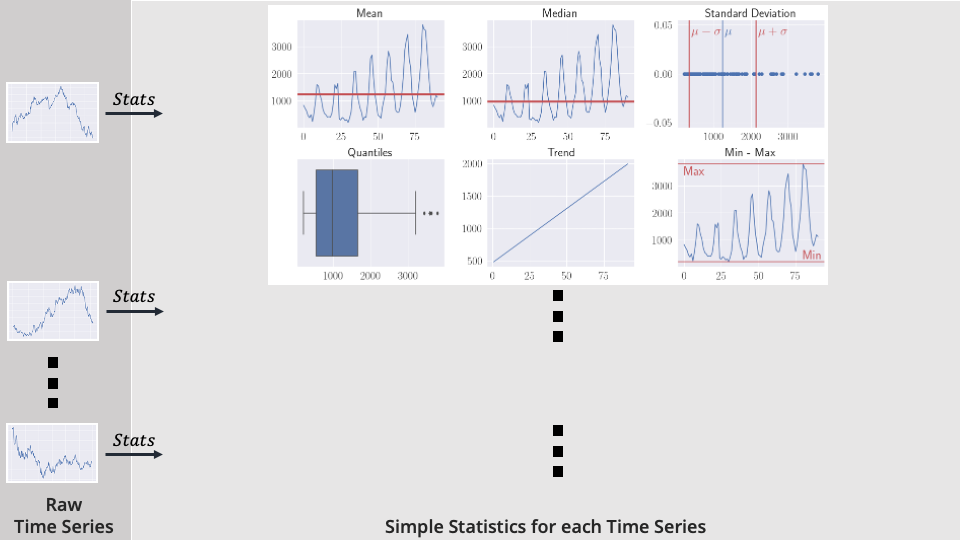
\includegraphics[width=.9\linewidth]{./img/process_simple_stats.png}
\caption{\label{fig:orgce8f2b5}Phase 1a: compute simple statistical metrics in time series pool for later comparison}
\end{figure}

As shown in figure \ref{fig:orgce8f2b5} the additional metrics are computed on the original time series, consisting of: (1) trend, (2) mean, (3) median, (4) standard deviation, (5) quantiles, and (6) minimum and max values. These metrics will be used flexibily to find similar series that match singular or multiple criteria. In essence the prior step of finding the underlying frequencies ensures that the time series follow similar periodicity or seasonality. The statistical metrics contain additional information that allow to find time series in the pool that, for example have similar value distribution through the standard deviation, etc and therefore match the users needs for the particular use case.

The trend mentioned above is not a strict statistical measure. However, we compute the slope \(m\) via linear fit of equation:
\begin{equation}
f(x) = m x + b
\end{equation}


Noteworthy is also the fact that the time complexity of the statistical metrics does not exceed \(\mathcal{O}(n \log(n))\). It of course depends on the sorting algorithms used for the computation. Assumming quicksort or mergesort this holds true. This observation also includes the computation of the linear fit which is \(\mathcal{O}(c^2 n)\) with \(c\) representing the number of features which. For our case \(c=1\), because we only have one feature or variable; hence time complexity for linear fit reduces to \(\mathcal{O}(n)\). This observation let's us conclude that the computation for the statistical metrics will be feasible during the similarity search for the template time series even if \(n\) is very large.
\subsection{Matching of time series}
\label{sec:orge7b944b}
\label{orgc5ae61a}
After the completion of phase I the time series pool is ready for use. When a new time series is to be matched against the pool first phase I for the individual time series needs to be executed as well, meaning the data transformation into frequency space and computation of the statistical metrics. First, for each of the of the Fourier transform types (regular, Hamming, Welch) the highest matching score (see section \ref{org93cfc1e}) between the template time series \(S_t\) and each of series in the pool \(S_n\) is computed via:

\begin{equation}
\argmax_{score\, \in \, S_{N}^{(type)}} f(score_{S_i}^{(type)}) = score_{S_i}^{(type)},
\end{equation}

where \(type\) refers to the FFT type. This reduces the pool of the matching series to all time series from the pool per FFT type that are equivalent to the highest matching score for that transformation type. The remaining series are discarded. Next an additional limitation is applied that restricts the result set of matching series (named \(A\)) to having a trend that must match in slope (up/down) to the slope of the template time series

\begin{equation}
A_{trend} = \{S_{i} \in S_{N} \mid \mathds{1}\left(- \frac{m_{S_t}}{\lvert m_{S_t} \rvert}
=- \frac{m_{S_{i}}}{\lvert m_{S_{i}} \rvert} \right)  \},
\end{equation}
where \(m_{S_t}\) is the slope of the template time series and \(m_{S_i}\) is the slope of the time series of the time series pool \(S_N\) currently under investigation.  This metric in our algorithm is used to rule out time series from the pool that have a trend that goes into the opposite direction of the template series. This property is not easily discernable from the coefficients found in the Fourier transform. For example if the series for which we want to find matching series in the pool has a negative trend, all series with a positive trend from the result set are ruled out before the other statistical metrics are utilized. However, if the trend for the investigation at hand is not relevant this step can easily be removed.

The last step in our algorithm to match series involves optimizing for one of the other statistical metrics computed on the original time series. With the metrics described in section \ref{orgfc6d82a} it makes sense to optimize for the lowest delta in desired statistical metric on the remaining result set after the previous matching steps. This selection is executed without regard for the transform method used as the metrics are comparable. The ranked difference between the template time series and the pool series is then used to select the most matching series
\begin{equation}
\argmin_{S_i\, \in\, S_N} f(S_i):= \lvert\phi_{S_t} - \phi_{S_i}\rvert
\end{equation}
Figure \ref{fig:org13e9cb3} provides a pictorial overview of the time series matching process.
\begin{figure}[htbp]
\centering
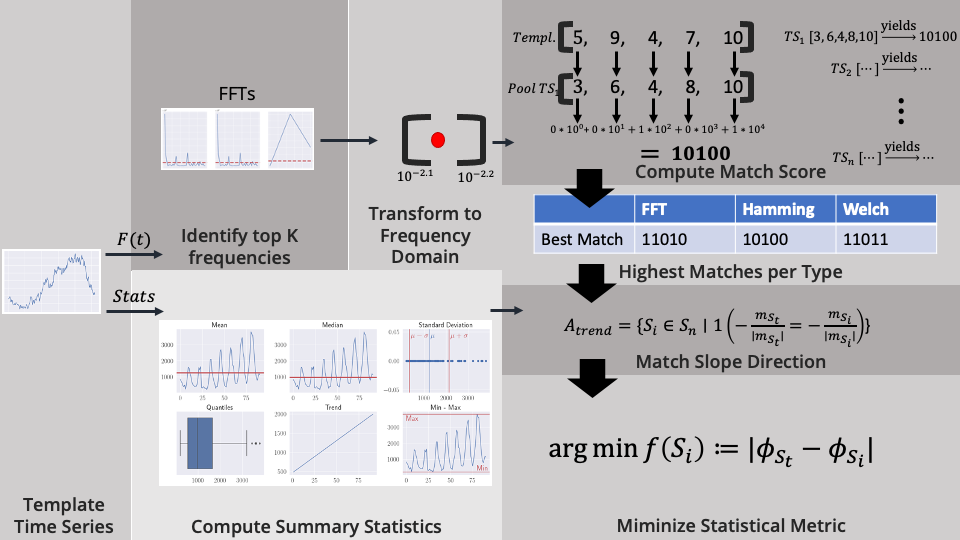
\includegraphics[width=.9\linewidth]{./img/process_match_ts.png}
\caption{\label{fig:org13e9cb3}Matching pool time series to template time series process}
\end{figure}

From the resulting order of the series one or multiple elements can be used to identify the most similar series to this algorithm. This can be done in multiple ways and is task dependent. This procedure does not impose some absolute truth in the results but rather a gradient of closeness that begins by the determining the frequencies contained in the Fourier domain as the most important descriptor of similarity between series. The remaining metrics then build upon the reduced result set to optimize for some aspect of similiarity between the series.

\section{Frequency handling in time series}
\label{sec:org5cbb63b}
\label{orgc3516ba}
\subsection{Frequency Ranges}
\label{sec:orged0367d}
\label{org9f9de98}
We want to be able to compare the closeness of two time series by comparing their frequencies with each other. Due to Parseval's Theorem (see section \ref{org8d4ed6b}) we know that properties of the raw series are partially preserved in the frequency domain. Equation \ref{org160dfd0} states that the energy contained in the norm of the frequency domain of the transformed time series is equal to the norm of \(f(x)\). The energy in the norm of the transform is proportional to the norm of \(f(x)\). What we can derive from that is that if there coefficients in the transform that are very small, they can be ignored without meaningfully impacting the result of the integral in the transform. Therefore, a truncated Fourier transform ranked by the magnitude of the coefficients will still remain a very good approximation to its original series. Additionally, because the Fourier transform is a unitary operator, meaning, it preserves lengths and angles in the frequency domain different series are comparable within in the Fourier space. So the distance between two time series is preserved in the frequency domain.

We utilize these properties by selecting the frequencies with the \(n\) largest magnitudes for a comparison. We select multiple frequencies and rather than computing the distance between each of the same-ranked frequencies we want to assign them to a range band that can be used to capture whether two time series have frequencies at the same rank that matches within a certain bandwidth. This is an approximation of the distance as frequencies will be determined to be similiar up to a certain distance and then be declared not matching.

A second observation is that lower frequencies have a larger impact on the overall shape of a time series then higher frequencies. Therefore, a match at lower frequencies requires a smaller band than a match at higher frequencies. To accomodate this observation the range band is defined by the set defined on a logarithmic scale
\begin{equation}
\Omega^{\prime}_n = \{ \omega^{\prime} = 10^\chi \in \mathbb{R} \mid \chi=k \cdot \Delta \; \land \; k \in \left[ \frac{a}{\Delta}, \frac{b}{\Delta}  \right], \quad
\Delta \in \mathbb{R_+}, \; k, a, b \in \mathbb{Z}\},
\end{equation}
where \(\omega^{\prime}\) denotes the identified frequency range and  \(\Delta\) is a fixed value defining the step size between the range intervals; \(a\) and \(b\) are the lower and upper limit of the interval(\(a < b\)). Generally \(k \ll a\) and \(k\) must be an integer value to delineate the range borders. An example can be seen in figure \ref{fig:org104a2c8}. For the figure a wider step change was chosen and the x-axis shown for both FFT and Hamming was limited to a smaller section so that the individual bins are and their associated values are visible.

\begin{figure}[htbp]
\centering
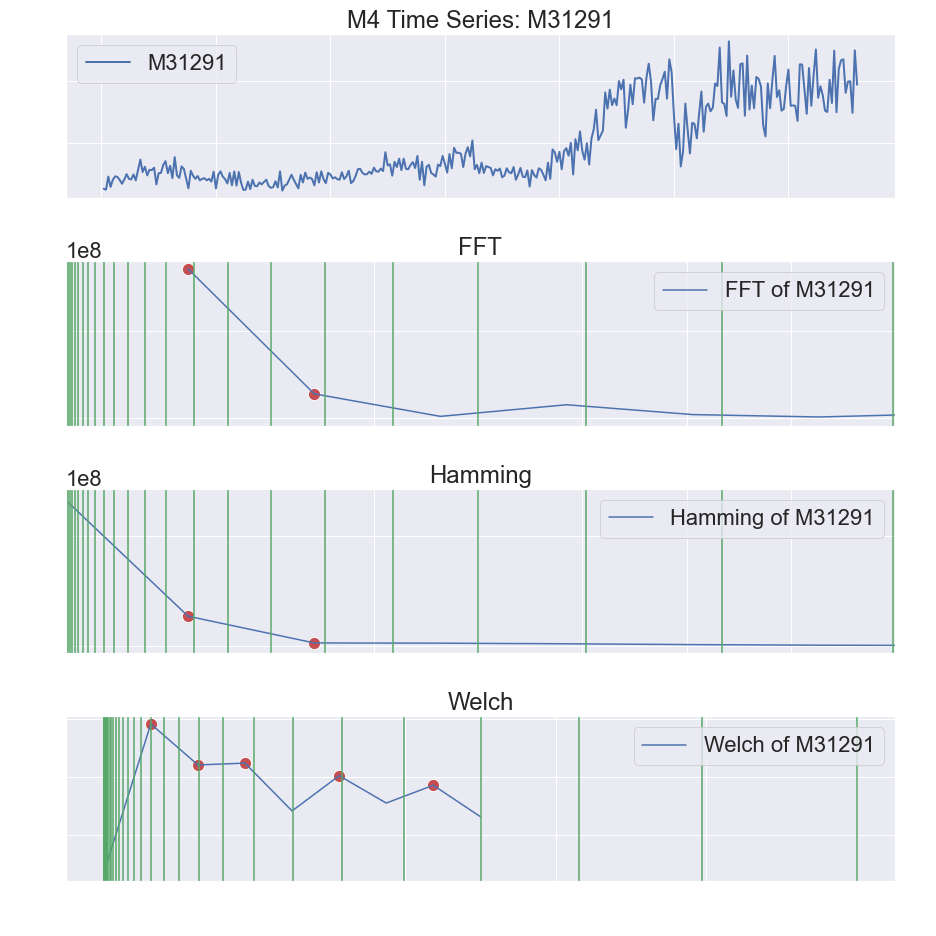
\includegraphics[width=.9\linewidth]{./img/freq_range_example.png}
\caption{\label{fig:org104a2c8}Frequency ranges definition - FFT example M4 data: M31291 with parameters \(a=10^{-4}\) to \(b=10^0\) with \(=Delta=0.1\)}
\end{figure}

For our work, we define \(a=-4\), \(b=0\) and \(\Delta=0.01\).

\subsection{Assigning frequencies to an interval}
\label{sec:orgb0f6e53}
\label{org772d555}
The top K frequencies need to be assigned to their respective interval. The association is done via this mechanism:
\begin{equation}
M_n(\omega)= n \mathds{1} \Omega^{\prime}_n(\omega) \quad \omega \in \left[\frac{a}{\Delta}, \frac{b}{\Delta}  \right].
\end{equation}
with \(\omega\) representing one of the top K frequencies identified via the FFT and \(\omega^{\prime}\) the respective representation in the frequency ranges set \(\Omega^{\prime}\). As an example, imagine a frequency identified via the FFT of \(\omega=0.003\) with \(a=-3\),\(b=0\), and \(\Delta=0.1\). The value of \(\omega\) falls into the interval \([10^{-2.6}, 10^{-2.5}]\). If \(\Omega^{\prime}\) is indexed from 0, the result will be \(M_n(\omega) = 6\).

\subsection{Matching frequencies between time series and ranking results}
\label{sec:org44f48f1}
\label{org93cfc1e}
To match the frequencies between time series a mechanism is required that considers the rank of the match within the top K frequencies. We use the another logarithmic scale with base 10 to signify the importance of the match which can later be used for ranking the results with
\begin{equation}
score = \sum_{k=0}^{K-1} 10^{k}\mathds{1}(\omega_{k}^{\prime \,(S_1)}) = \omega_k^{\prime \, (S_2)}
\end{equation}
where \(\omega_{k}^{\prime \, (Sn)}\) represents the k\textsuperscript{th} ranked frequency band \(\omega^{\prime}\) of time series \(S_n\). The score is computed for each time series in the time series pool for each transform, meaning regular FFT, FFT with a Hamming window, and FFT with Welch's method using a Hamming window.

For each transform type all series are ranked based on their matching score in descending order. A higher score means that the more dominant frequencies in the series match. In the algorithm all time series from the pool that have the highest match score per transform type are selected for further processing that utilize the statistical metrics.

\section{Main contribution of the thesis}
\label{sec:orga9ed9eb}
\begin{itemize}
\item transformation into Fourier-space
\item transfer frequencies into frequency range band with increasing range width (using log scale)
\item computation of frequency energy levels (sort and keep top 5) -> ask Prof. how to name this parameter
\item conversion of ordered frequencies into frequency range band
\item for each series to compare -> compare whether the frequency matches on the ordered positions -> provide exponential value per position -> match on more powerful frequencies is valued higher
\end{itemize}
\section{additional computations}
\label{sec:org027ed4d}
\begin{itemize}
\item utilization of FFT utilizes only frequency space (future work should consider comparison of energy levels per frequency)
\item additional simple statistics computed (mean, std, quantiles)
\item ts decomposition for trend estimation (requires parameter for period) -> then best line fit for slope of the time series
\item computation of deltas for each series to search with statistics and slope of all other time series (review computational complexlity)
\item ranking of matching series based highest frequency range match and ONE statistic
\end{itemize}
\section{Preprocessing}
\label{sec:org3374f0f}
\begin{itemize}
\item M4 data wide format vs. long format
\end{itemize}
\section{Parallelization}
\label{sec:org2a864fc}
\begin{itemize}
\item computation times
\item scalability
\item Samples for results only (stratification vs. non-stratification)
\end{itemize}
\begin{enumerate}
\item Threads vs. Processes
\label{sec:org63c8c19}
\end{enumerate}

\section{Technology (check with Prof. if required)}
\label{sec:org0559003}
R vs. Python vs. Mathematica, Matlab
\begin{itemize}
\item all languages have FFT either built in or available through common packages
\end{itemize}
\section{}
\label{sec:org1e04724}
\begin{itemize}
\item load
\item transform to FFT vector space
\item compare most important frequencies
\item compare candidates
\item select winner (which criteria)
\end{itemize}
\chapter{Data Analysis}
\label{sec:org693a181}
To develop a method to find similar time series in a pool of time series a replicatable data set is required that ideally represents real-world scenarios from a wide range of fields with differing time granularities. In the literature two widely used datasets can be found which will is introduced in sections \ref{org44d15b1} and \ref{orgfc20129}. For the process of developing the FFT-based similarity detection method the M4 competition data was used \cite{M4CompetitionArchive2018}. All parameter choices were done with the exploratory data analysis results of the M4 data. To verify their veracity the formal evaluation of the method results were conducted with UCR Time Series Classification Archive \cite{UCRArchive2018}. This was done ensure that the results found and parameter choices made are applicable between different data domains and time granularities, as well as providing reference points for quality of the method described in this thesis.

\subsection{M4 competition data}
\label{sec:orge8e33b8}
\label{org44d15b1}
In his popular book "The Black Swan - The Impact of the Highly Improbable" published in \citeyear{taleb2008black} the author \citeauthor{taleb2008black} introduced the M-competitions and its merits to an international readership. By that time already 3 M-competitions were already conducted with the first one done in \citeyear{makridakis1982}. \citeauthor{makridakis1982} held the forecasting competition as a follow-up to a controversial paper published in \citeyear{makridakis1979}. In the paper \citeauthor{makridakis1979} found that more sophisticated forecasting methods tended to lead to less accurate predictions, a view for which he highly criticited and personally attacked. The forecasting competition was an answer to the accusations to allow the experts to fine-tune their favorite forecasting methods to the best of their knowledge and compete for the most accurate predictions on the hold-out set \cite{makridakis1982}. The competition was based on 1001 different time series and provided an inside into the different properties of the various used forecasting methods. The data itself was selected with varying time granularities, different start and end times. It was chosen among data from different industries, firms and various countries. It consisted of macro-economic and micro-economic data. The results observed in the earlier work from \citeyear{makridakis1979} was confirmed in the forecasting competition. The main observations were that stastically sophisticated methods on average provided not more accurate forecasts than simpler methods and accuracy improvement can be achieved by combining the results from various different methods \cite{hyndman2020}.

With the M4 a random selection of 100,000 series was performed by Professor Makridakis and provided for the forecasting competition in 2018. It included data with a time granularity ranging from hourly, daily, weekly, monthly, quarterly, and yearly data. It came from various areas: micro-economical, industrial, macro-economical, finance, demographic and miscellaneous areas \cite{makridakis2020}. This a wide field of mostly socio-economic data with varying time granularities, different time series length. What is not present or possibly underrepresented in the dataset are time series generated by technical processes, like machine or sensor data. Nonetheless, these time series data are an ideal candidate to develop and test and method for discovering similar time series. This time series archive was chosen as the dataset to develop the algorithm of indentifying similar time series quickly based on their Fast Fourier transform.

The latest completed  iteration of the Makridakis-competition is the M5 \cite{spiliotis2021}. It was completed in 2021 and was set up with product sales in 3 different states in 10 different stores in the United States. It consisted of the sales of 3490 different products sold by Walmart. The data came from the identical time frame ranging from 2011 to 2016. Due to the similar nature of the data contained in this dataset it was ruled as the basis for our investigation.

At the time of this writing in fall 2021, the next installment of the Makridakis-competition, the M6 is in planning to be conducted starting in February 2022.
\subsection{UCR time series data}
\label{sec:orgab7b219}
\label{orgfc20129}
Another important dataset with an even broader usage in time series research is the UCR Time Series Archive. It was first formed in 2002 by Prof. Keogh \cite{hoang2019}. It's intention was to provide a baseline for time series research which prior to that point mostly relied on testing a single time series per paper. The creators concluded that this makes comparing the results between papers almost impossible. The dataset was expanded in the subsequent decades with the last major expansion being conducted in 2018.

In his \citeyear{keogh2003} published paper \citeauthor{keogh2003} describe the error of data bias which comes from testing new methods on a single time series or time series of the same kind, for example ECG data but extending the claim of the found results to various types of time series data or all time series data types. With this in mind the UCR Time Series Archive was compiled and subsequently extended with various time series from various areas including: (1) Image, (2) Spectro, (3) Sensor, (4) Simulated, (5) Device, (6) Motion, (7) ECG, (8) Traffic, (9) EOG, (10) HRM, (11) Traffic, (12) EPG, (13) Hemodynamics, (14) Power, and (15) Spectrum time series data. This is a wide spectrum of data which is different from the socio-economic data of the Makridakis competition datasets. Therefore, this dataset is a great candidate to validate the findings of the time series similarity search and conduct a formal evaluation of the results found via the M4 dataset. Furthermore, it provides a classification category for each time series dataset which in itself is made up of multiple time series. In this way running a formal evaluation, we can measure how many datasets are identified between the train and test set of the data that belong to the same dataset and dataset class. This metric can then be compared between the Dynamic Time Warping (DTW) algorithm and our method.
\subsection{Exploratory data analysis}
\label{sec:orgb1d9065}
\label{orgd07bcf6}
In order to be able to set parameters for the the utilized methods in the data transformation (see section \ref{orge0cee10}) and the computation of the statistical metrics (see section \ref{orgfc6d82a}) an understanding of the used data is necessary. Please note, that the decision for parameters was done based solely, on the M4 competition data set (section \ref{org44d15b1}) and the UCR data set was only introduced during the formal evalution (section \ref{orgfc20129}).

The first analyzed aspect is the length of the time series in the two repositories. In figure \ref{fig:orgd8e9d3b} can see that the lengths of the two repositories time series have different distributions. For the M4 dataset has the wider range of \([13, 9919]\) while the UCR dataset is distributed between a length of \([8, 2844]\). For the M4 dataset the data is more concentrated around the length of roughly 100 data points and a second peak at 320 data points. Further there are some time series with longer series concentrated around 4000 datapoints.The mean is 240 datapoints and the median is 97, meaning there are some outliers on the longer side of the distribution. This is confirmed by the boxplot of the lenghts of the two repositories (see figure \ref{fig:org254ae4b}). The UCR repository doesn't have as many short or long series compared to M4. The main concentration is simlilar to M4, with a bimodal distribution around roughly 100 data points and a second higher peak at 650-700 datapoints. But the lengths are more concentrated in that region, confirmed by lower standard deviation of the UCR dataset compared to the M4 data.
\begin{figure}[htbp]
\centering
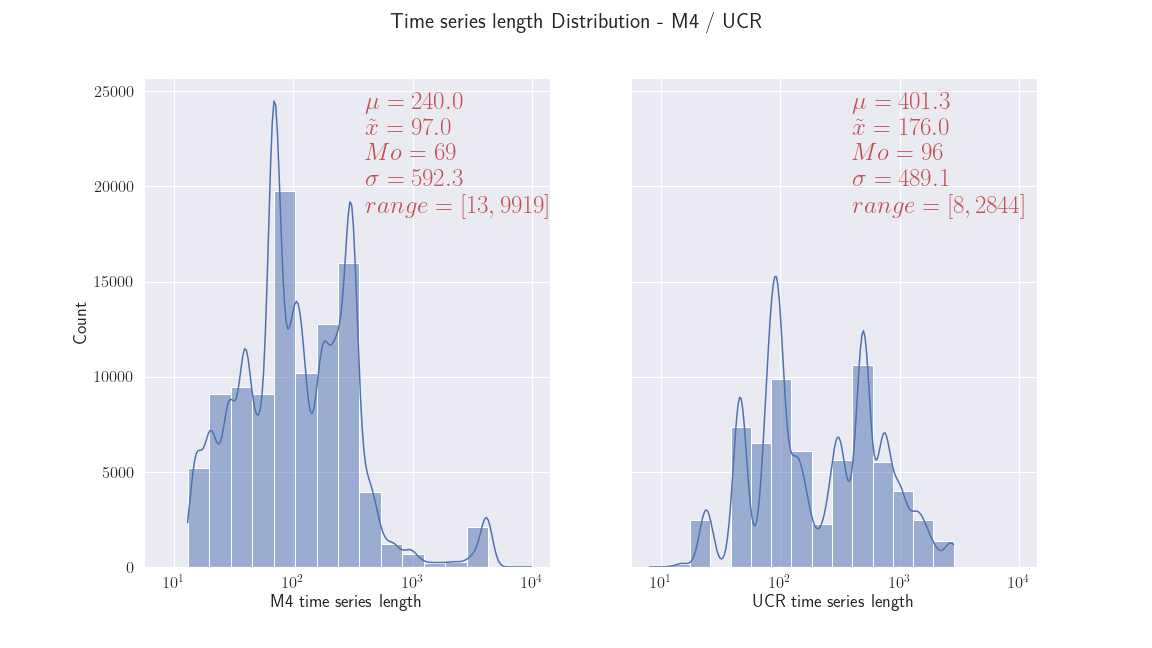
\includegraphics[width=.9\linewidth]{./img/ts_m4_ucr_length.png}
\caption{\label{fig:orgd8e9d3b}Histogram / KDE of time series length in repositories}
\end{figure}
The UCR data is also impacted by a few outliers leading to a higher mean than median as can be seen in the boxplot. But this is less so compared to the M4 data which has roughly have of the mean and median value to the UCR data.

\begin{figure}[htbp]
\centering
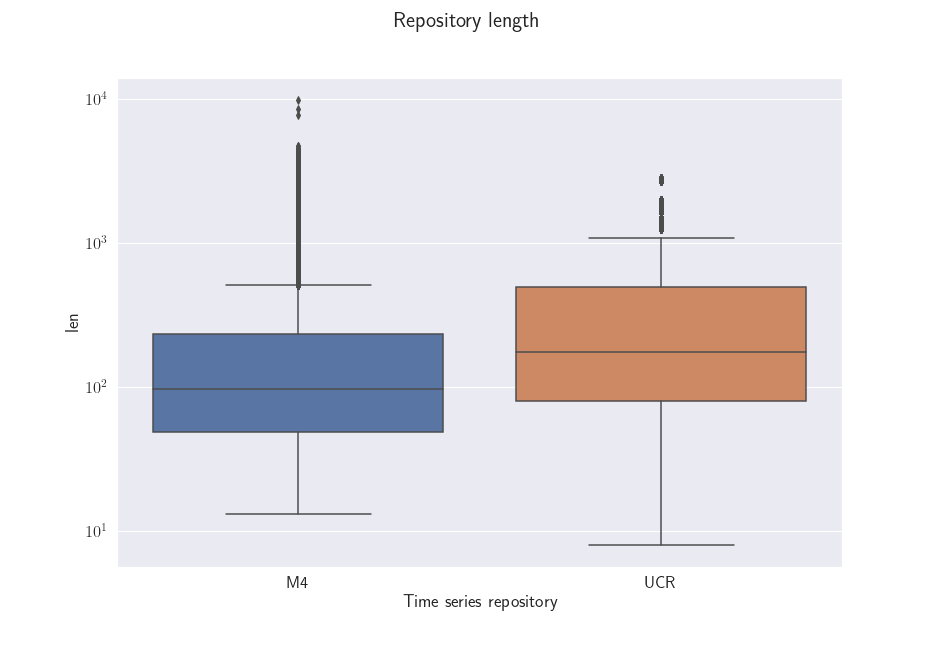
\includegraphics[width=.9\linewidth]{./img/ts_len_m4_ucr_boxp.png}
\caption{\label{fig:org254ae4b}Boxplots of M4 and UCR time series length}
\end{figure}

These observations are interesting for multiple reasons. For one, they will reveal whether the devised method for finding similar time series works equally well irrespective of the length of the underlying pool time series. Furthermore, the data can be used to illustrate the compression levels achieved in the computation of the similar time series via the FFT. For the M4 dataset with a \(\mu=240\), the reduction to the top 5 frequencies for the comparision with other time series leads to 60x reduction in data points required for comparison. The longest series in M4 is reduced by factor 1980. Aside from the algorithm being in a favorable time complexity class of \(\mathcal{O}(n\log(n))\) also a constant term of very few datapoints is required for the comparison in the Fourier domain. The compression is even more favorable in the UCR dataset. The \(\mu=401.3\) datasets lead to a compression factor of 80x on average.

The next area of analysis is the value distribution of the time series both in UCR and the M4 repositories. As can be seen in figure \ref{fig:org753dac7} the values in both data repositories are distributed very different. The M4 dataset has more times series than the UCR dataset, \(100000\) vs. \(\approx 65000\). But the UCR dataset contains on average longer series totalling about \(\approx\) 26 million datapoints, compared to \(\approx\) 24 million datapoints for the M4 dataset. The distribution of those data points is over a wider range for the M4 repository, spanning \([10,703008]\). In contrast the UCR dataset covers the range of \([-1110.8,24929]\) including negative values but covering a mucher smaller spectrum of values. This is reflected in the mean values for both repositories, for M4 \(\mu=4841\) and for UCR \(\mu=7.96\). Both distributions respectively contain large positive outliers and therefore the median values are lower. M4 has a median of 3689, while for UCR the median is 0.00137. The difference of the distribution can also be seen in the different standard deviations of both distributions. M4 has a \(\sigma=5724\) and UCR has \(\sigma=99.67\).

\begin{figure}[htbp]
\centering
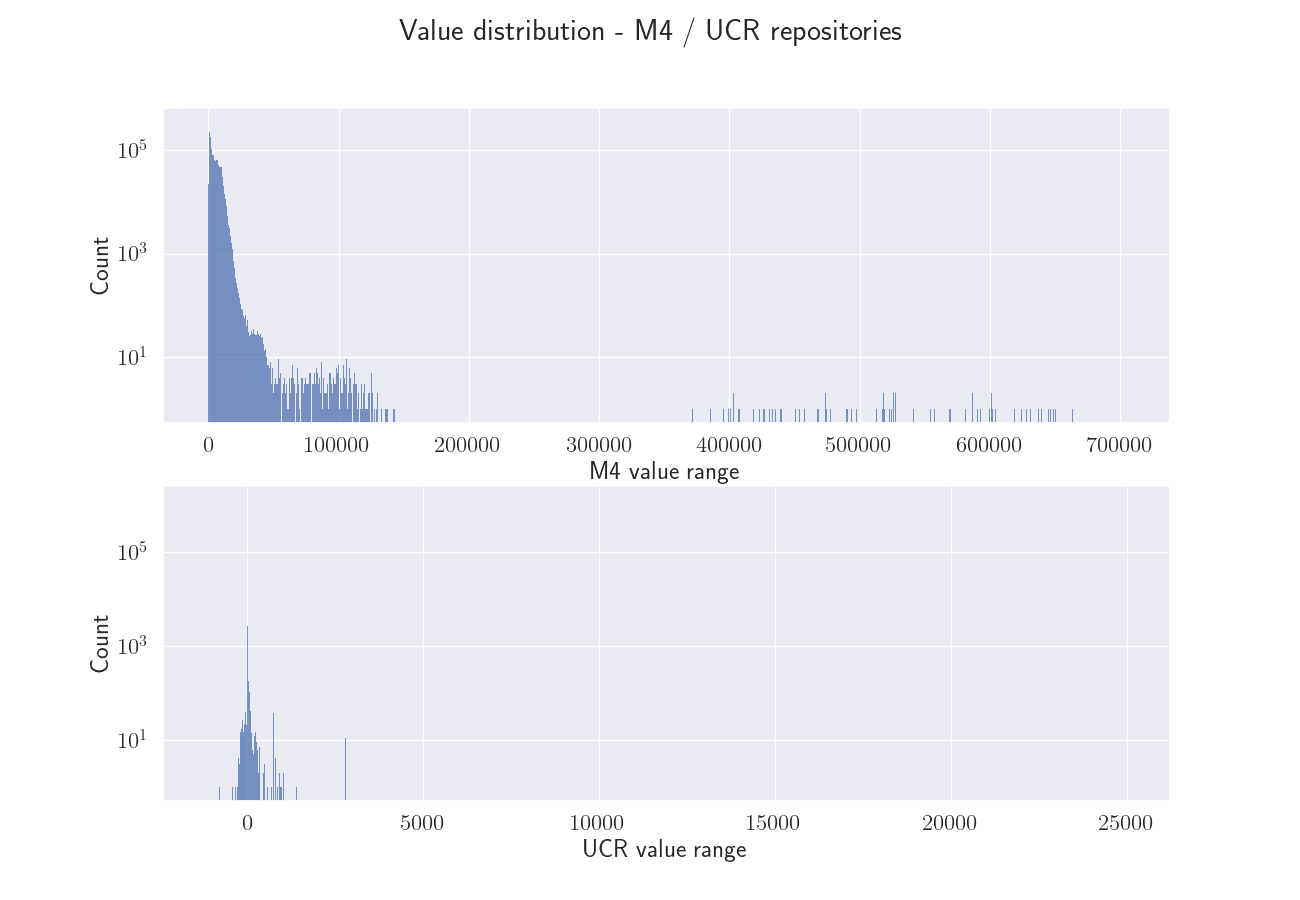
\includegraphics[width=.9\linewidth]{./img/m4_ucr_val_hist.png}
\caption{\label{fig:org753dac7}Value distribution for M4 and UCR data repositories}
\end{figure}

Another interesting area of comparison is the distribution of the two data repositories in the Fourier domain. The distribution of the top 5 frequencies for M4 and UCR data sets can be seen in figure \ref{fig:orge02d9fb} setup with a log-scale for the y-axis. We observe that the frequency distribution differs between the two data sets. First, we notice that the distribution of both the regular FFT and Hamming FFT are similar in both datasets. However, for the M4 data the Hamming windows the middle of the frequency spectrum around 0.5 shows a higher concentration of frequencies compared to the regular FFT. This is not observable for the UCR dataset. Overall, the distribution for the UCR dataset is more smoothly distributed compared to the M4 data. Possibly, this can be explained by the fact that the data in the M4 data is more socio-economic data leading to more erratic datasets compared to the more technical time series from the UCR repository, where more regular patterns are observable. For both repositories a rise of frequencies along the edges can be seen. Especially the left edge at the lower frequencies is very important because the lower frequencies have a higher impact on the overall shape of the resulting time series. Therefore, a more granular setup of ranges is beneficial for the comparison of the series, as described in section \ref{org772d555}. Noteworthy is also the distinct difference between the Hamming and regular FFT frequency spectrum on the one side and the Welch's method frequencies on the other. The averaging of the subsegments leads to overall lower frequency values. It also visualizes why the intra-FFT-type frequency comparison would result in misleading results.

\begin{figure}[htbp]
\centering
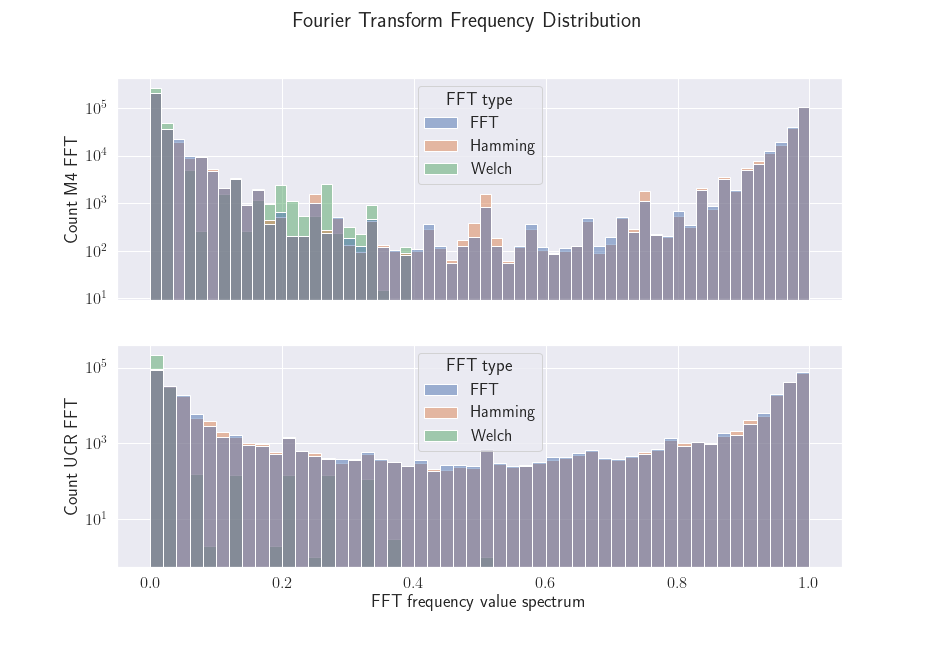
\includegraphics[width=.9\linewidth]{./img/fft_freq_dist_ucr_m4.png}
\caption{\label{fig:orge02d9fb}FFT frequency distribution for M4 and UCR dataset}
\end{figure}

A further drilldown into the distributions reveals more differences between the two data repositories which can be observed in figure \ref{fig:org67cf7ce}. Here, the frequency distributions are shown by rank of of frequencies. For example, row 1 in the plot indicates the distribution of the highest ranked frequencies by transform method separated by the M4 repository on the left and the UCR dataset on the right side. We observe that different data makeup between the two repositories is even more obvious than before. For example, the M4 dataset has a narrow distribution of frequencies ranked at the top stop. In fact, Hamming and regular FFT are exclusively zero and only the Welch's method has some spread, likely due to the averaging of the segments. Another, explanation are the higher average values of the M4 dataset which requires a different y-axis offset. This is accomplished via frequency zero which results just in a flat line when inverse transformed from frequency domain to the original domain. The top 2 ranked frequncies for the M4 dataset span the whole range of frequencies but a different distribution between the transform types can be observed. The Hamming FFT is found at the left and right edges whereas the regular FFT frequencies are distributed smoother with an increase towards the higher range of the frequency spectrum. The data is consistently occupies a smaller range between \([0.1,0.4]\). For the UCR repository the distribution is comparable to the first ranked frequencies with a sharper dropoff in the middle of the frequency domain. Rank 3, 4 and 5 repeat the previous patterns of the respective distributions for M4 and UCR data. The most notable differences are the general deviation between the M4 and UCR repository and second that rank 4 for the UCR dataset has the largest amount of frequencies gathered around zero for Welch's methods frequencies.

\begin{figure}[htbp]
\centering
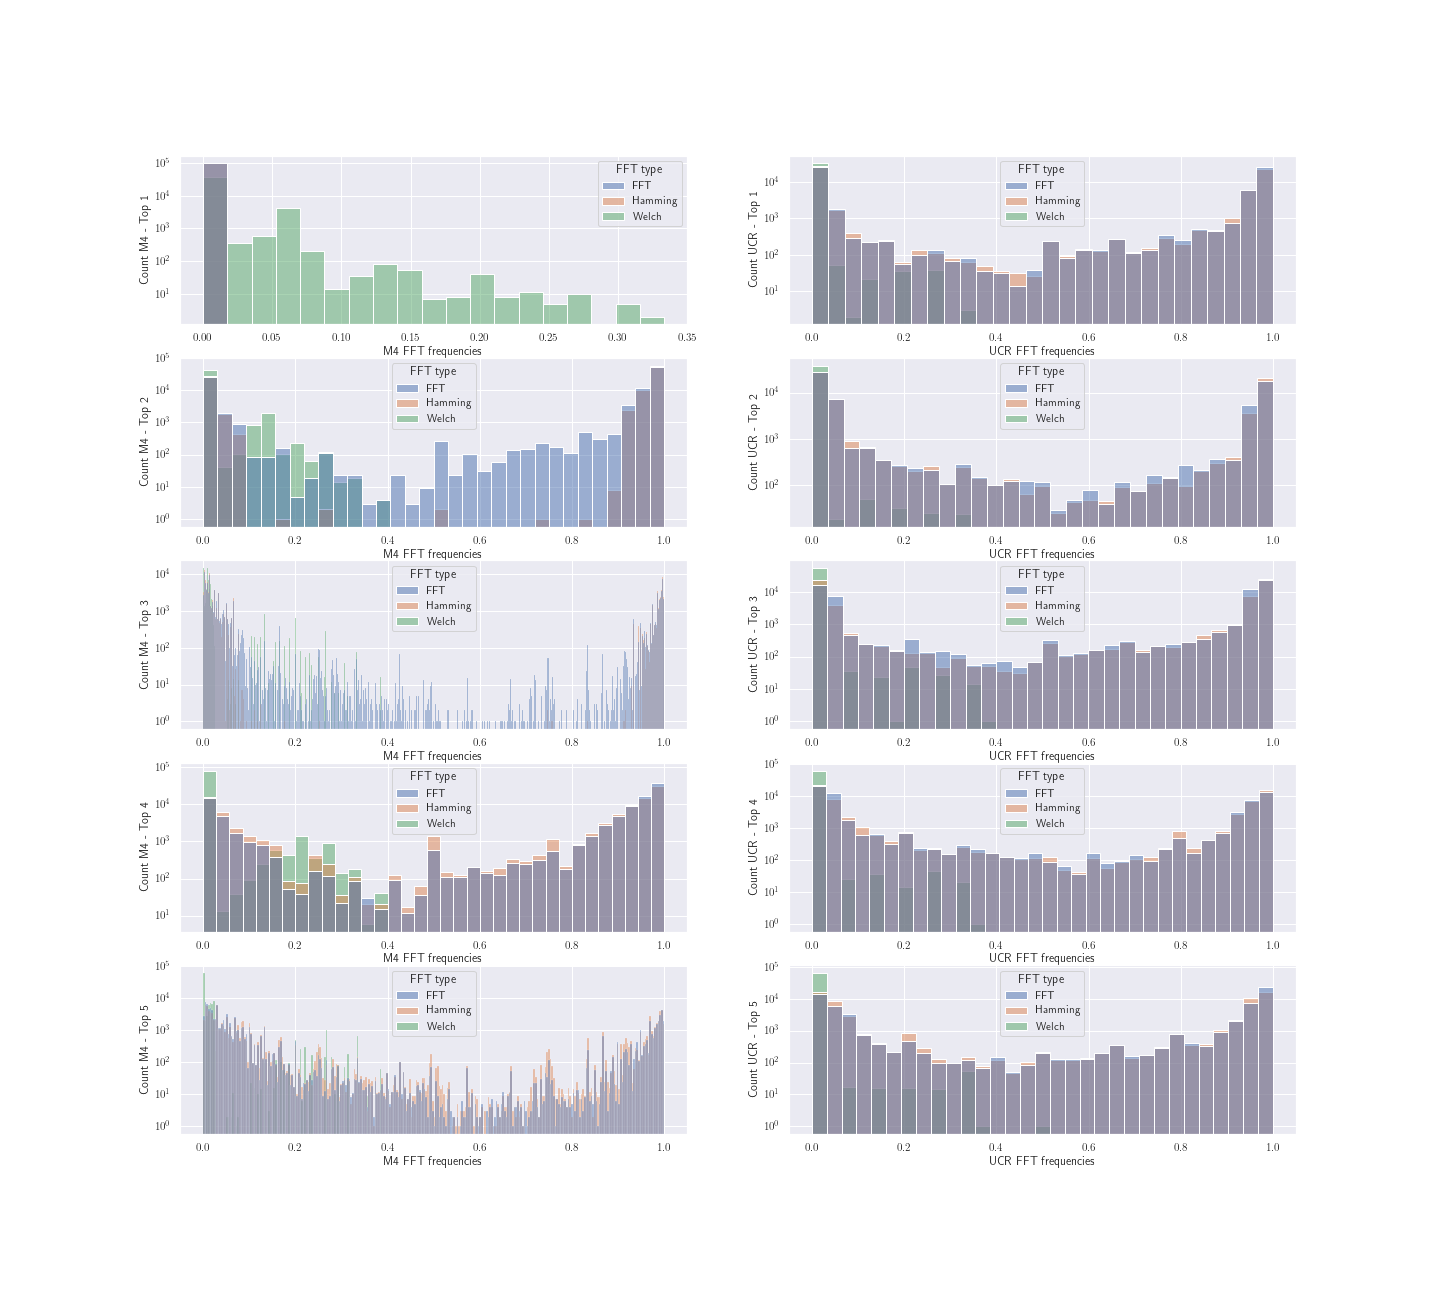
\includegraphics[width=.9\linewidth]{./img/fft_freq_topk.png}
\caption{\label{fig:org67cf7ce}FFT frequency distribution by top k for M4 and UCR dataset}
\end{figure}

The review of the ranked frequency distributions does not reveal any information that indicates that the ranks should be treated differently from the process defined in section \ref{orgc3516ba}.

\chapter{Formal Evaluation}
\label{sec:org0b7c0b6}
The formal evaluation covers the following aspects aims to establish a formal comparision between the algorithm presented in this work compared to the widely used and generally accepted method of Dynamic Time Warping for finding similar time series. We will introduce the evalution method chosen, discuss the consequences of the different time complexities of the algorithms, and compare the accomplished results via the two methods.

\section{Evalution Method}
\label{sec:org87ab00a}
To evaluate the performance of the algorithm proposed in this work the following procedure was applied to the UCR time series data set. To generate the results with our the method the whole data set was transformed and augmented as described in section \ref{orge0400ec}. After the transformation and stratified random sample of 1420 was chosen from the UCR test dataset, such that each different data repository inside UCR dataset is represented.

The resulting data test time series have then been processed by both algorithms Dynamic Time Warping (DTW) and the algorithm described in section \ref{orge0400ec}. The DTW method has been used been introduced by \citeauthor{giorgino2009} which was implemented via a statistical software package in R \cite{giorgino2009}. The only change to the standard call of the method was the utilization of the option to only compute the distance and not generate any data for plotting the data to improve the runtime. The random sample was run over the time series pool of all training data irrespective of the category the data was chosen from. For the DTW method the closest match from the time series pool was recorded. This results in one closest match per time series from the sample.

For the FFT-based method to find similar time series the procedure was similar in that each time series from the sample was compared to all series from the time series pool of all training time series. Because there are multiple metrics on the window side with the regular FFT, Hamming and Welch's method and the different summary statistics the lowest result for each combination was recorded. To illustrate, each time series converted to each window type, for example Hamming each KPI (mean, median, standard deviation, etc) was recorded based on the closest \(\Delta\) value. So per time series and window type 8 minimized KPI values were recorded.

With these results the performance evaluation was conducted.
\section{Time complexity and duration}
\label{sec:org3a965c2}
Due to the different time complexities of the underlying algorithms two different computers were used for the execution. Both algorithms were parallelized to allow to utilize more powerful compute infrastructures. The FFT-based algorithm was executed on a personal laptop 8 Intel-based CPU, 16GB RAM machine that simulataneously also ran other user-based activities. For the DTW a cloud-based machine with 32 CPU and 64 GB of RAM was chosen. Comparing the actual runtimes on these different hardwares and different operating system is not a good scientific measure of performance but is provided here to give an indication of the class difference between the two algorithms. The DTW required 2.9 days of execution time on the cloud hardware, compared to 22.5 minutes for the FFT-based algorithm. The DTW method was only executed once, therefore no repeated measurements have been taken to confirm the execution time of the entire dataset. However, repeated measurements have been taken to evalute the performance of finding the best match for a single template series in the UCR time series pool. The results vary depending on the length of the time series but average 180 seconds for the UCR time series pool in our Python implementation. This operation is not parallelized but is executed on a single core. For the FFT-based algorithm computing the results for single template series across the UCR dataset averages given all windows takes roughly 0.016 seconds on the 8-core machine. The results for the entire test set was run with parallelization but the search for one template series is executed on a single core. The difference amounts to an performance difference factor of roughly 11.250. The given results for the execution time include additional computational complexity as well as wait times for writing files to the hard drive. Those additional steps are more for the FFT-based scenario and could be left out if we are not interested in analyzing the intermediate steps. This would further increase the time performance advantage of the FFT-based method.

To generalize these is results it is pertinent to look at time complexity of the two algorithms. For this multiple things need to be reviewed. For Dynamic Time Warping the case is straightforward, because only \(\mathcal{O}(m*n)\) needs to be considered for the number of \(l\) series in the time series pool for:
\begin{equation}
\mathcal{O}(\sum_{i=0}^l (m_i*n))
\end{equation}
The similarity search proposed in this work has two multiple components consisting of the transformation of the time series, computing the summary statistics and running the comparison. The transformation of the series to the frequency domain is combined with the computation of the summary statistics including also the linear fit to find the slope of the series. It can be noted as:
\begin{equation}
\mathcal{O}(o (n \log n) + p n)
\end{equation}
with \(p\) being the number of computations that have complexity \(n \log n\) and \(p\) the number of computations having complexity \(n\). Of course, the constants are ignored and only the worst term is kept for the asymptotic behavior of this step resulting in:
\begin{equation}
\mathcal{O}(n \log n)
\end{equation}
For the second step we rank compute the matching score of the frequencies. This is special insofar as the time complexity linear with \(\mathcal{O}(n)\) and \(n\) being the number of frequencies to be compared. However, for our analysis this \(n\) is constant as we are only comparing the top \(k\) frequencies. This step is done for all series in the time series pool leading to:
\begin{equation}
\mathcal{O}(\sum_{i=0}^l (k))
\end{equation}
Next the delta's between the template time series and each pool time series needs to be computed:
\begin{equation}
\mathcal{O}((o+p-1)l)
\end{equation}
with \(o\) and \(p\) still representing the number of summary statistics in each time complexity class and \(-1\) because the comparison of frequencies is already captured. The last step is to filter and sort the result set which can be described by the time complexity of a sorting algorithm:
\begin{equation}
\mathcal{O}(l \log l)
\end{equation}
Combining these steps, removing constants and keeping the worst component per variable the time complexity of our similarity search can be described by:
\begin{equation}
\mathcal{O}(l \log l)
\end{equation}
Looking at the individual parts it makes sense that our method is most impacted by the size of the time series pool whereas DTW is impacted by both the size of the pool and the length of the series to be compared.

To be able to visualize the impact of these results we simplify the time complexity of DTW with the assumption that \(m_i = n\), meaning that all time series have the same length. This changes the time complexity of DTW to:
\begin{equation}
\mathcal{O}(l n^2)
\end{equation}
We now have only two input variables for the time complexity with \(n\) being the number of data points and \(l\) the number of series in the pool. The visualization of FFT-based algorithm only has \(l\) as input variable and could be done with a 2d-dimensional plot. However, to be able to compare with DTW will print it separately with 3D plot to reveal its general shape (see figure \ref{fig:orga1fc5ee}). We see the log-linear growth of the compute time that is respective of the length of \(n\).

\begin{figure}[htbp]
\centering
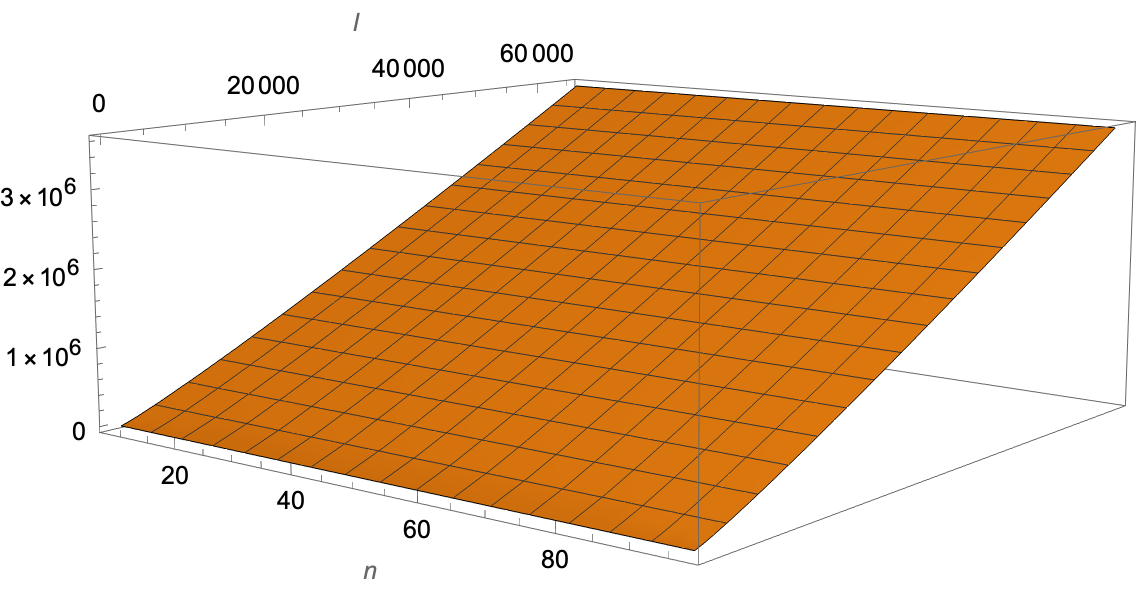
\includegraphics[width=.9\linewidth]{./img/tc_fft.png}
\caption{\label{fig:orga1fc5ee}Time complexity of our FFT-based similarity search}
\end{figure}

When visualizing the time complexity of our similarity search algorithm (orange) together with the time complexity of the DTW algorithm (blue) the difference becomes obvious the more we approach the actual values that represent the UCR data set, meaning \(n = 401\) and \(l \approx 65000\).
\begin{figure}[htbp]
\centering
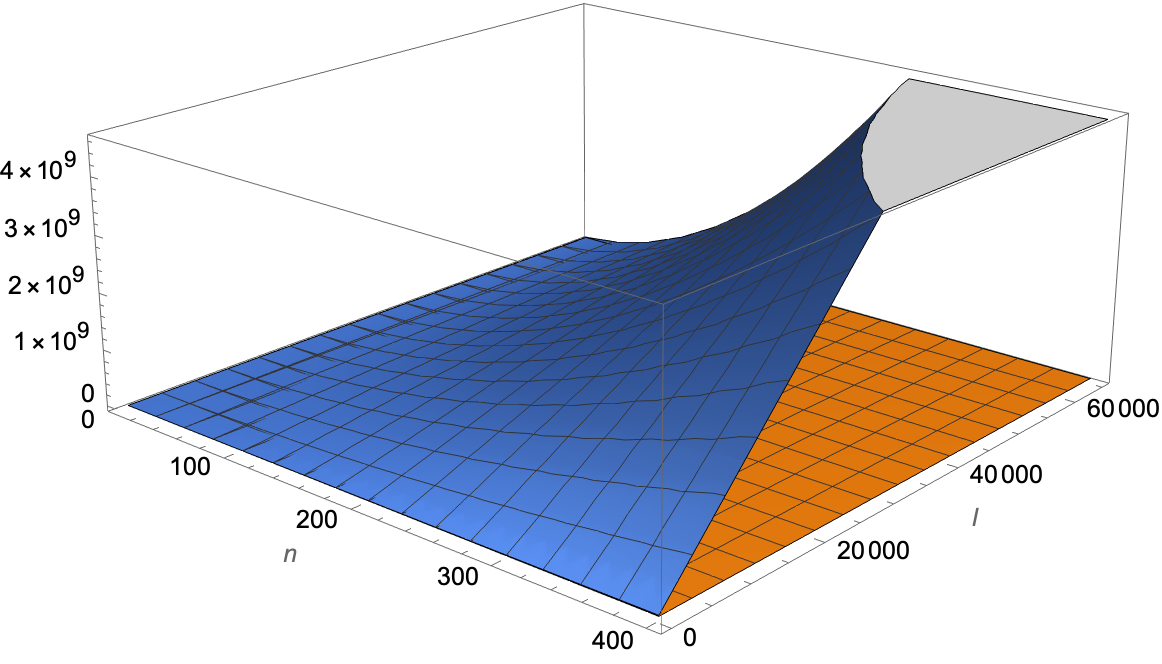
\includegraphics[width=.9\linewidth]{./img/tc_dtw_fft.png}
\caption{\label{fig:org9b562ea}Time complexity of DTW and FFT-based algorithm}
\end{figure}

It is obvious that performance of our proposed method significantly outperforms the DTW-based method. In real-world scenarios this already true for very small values of \(n\) and \(l\).

\section{UCR results overview}
\label{sec:org1665f87}
\label{org6276c12}
The UCR dataset provides a unique property that is interesting for a formal evaluation. Each time series in a category, for example ECG5000 in the test data is assigned a class value \cite{hoang2019}. The way of classification of the time series is different between the different time series data categories in the repository. For example \citeauthor{willet2016} utilizes other published standards to classify the data into feeding states of insect vectors \cite{willet2016}. This time series repository is part of the UCR archive. In consequence, the data overall follow different principles for classification that cannot be generalized into a single method.

For Dynamic Time Warping in 63\% of the cases (889 out of 1420) from the random sample was found within in the same data category. And from those within the same category  74\% of the time series (658/889) where attributed to the same class. 112 categories of 128 original categories in the random sample have a match within the same category.

The results for the FFT-based time similarity have some similarities to the DTW results. The random sample of 1420 time series taken from the test set produced 823 cases of the same data category as result for the best window type and KPI combination (Welch and standard deviation). Recall, that for with the FFT-based method each series is transformed via 3 different window types and augmented with 8 summary statistic KPIs available for selection. This produces 24 results per time series from the random sample. This is indicative of an observation one can make when checking multiple samples of the matching series (see \ref{orga341cff}). Very often the series found via the FFT-based method have a very similar shape and value level to template series and are comparable to the results achieved via the DTW. Important to note is that in order to keep data volume required for comparing the match scores at a reasonable file size a threshold for the match score was introduced. It was set to 10\textsuperscript{3} as the minimum score to be needed to be allowed to be considered a match. However, the lowest score match was 11001 or 10\textsuperscript{4}+10\textsuperscript{3}+10\textsuperscript{0}.

\begin{figure}[htbp]
\centering
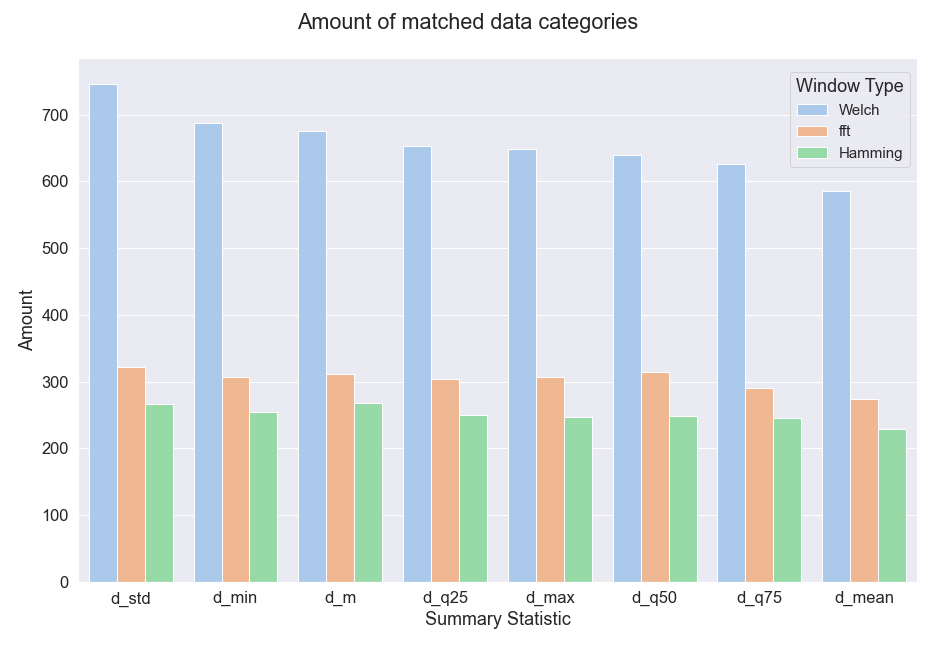
\includegraphics[width=.9\linewidth]{./img/fft_matched_cats.png}
\caption{\label{fig:orgd44a1fc}Number of matched data categories in UCR repository}
\end{figure}

Noteable is the distribution of the different window types is that their distribution between the different statistics is somewhat random with Welch's window having both the highest total of any metric with standard deviation (823) but having the least in all other categories. And FFT and Hamming are very similar in all categories with the biggest deviation in the trend category. Also interesting to observe is that quantiles, min, and max values tend to perform better to identify the same data category compared to trend and mean.

Where the results between the DTW and our approach differ are in the identification of the classes assigned to the time series. In figure \ref{fig:org22b36a8} one can observe the distribution of matched classes of time series. Of course, this requires that also the data categories are matched. With 41 matches for the combination of Hamming FFT and the series trend as summary statistic this results only in a 5\% match of the 755 matches from this analytics combination. Analogous to the data categories, Welch's method is most adequate for finding the same class when contrasted with the other window functions. From the summary statistics the best performing metric is the trend measure to identify the same class. It performs 2.7 times better than the second best measure. This information is useful in to decide which metrics to use when trying to identify the same data class. However, the overall performance of our algorithm is not sufficient to contest the results of Dynamic Time Warping.

\begin{figure}[htbp]
\centering
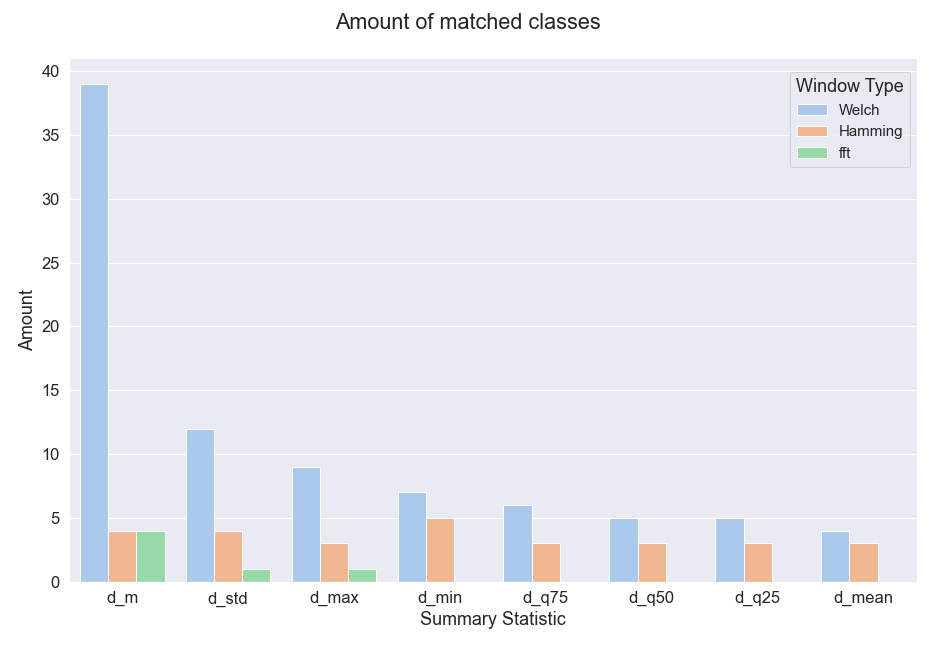
\includegraphics[width=.9\linewidth]{./img/fft_matched_cls.png}
\caption{\label{fig:org22b36a8}Number of matched classes in UCR repository}
\end{figure}

A visual inspection of the results produced by the different windows and summary statistics (see \ref{orga341cff}) shows that the overall performance of finding similar time series is good with intermittent mishaps. For example figure \ref{fig:org0c72bc6} and figure \ref{fig:org4449995} are good examples of the capabilities of our proposed approach.

Nonetheless, there are other examples were some summary statistics have good results but others produce bad results. See for example figure \ref{fig:org54549bb}. The data analysis in section \ref{orgd07bcf6} showed the increase of frequencies at the low and high end. Possible remedies could be linear range setup that increase the compute time, or using classical clustering metrics like Euclidean distance of the ranked frequencies, or creating a range that is sensitive on the low and high boundaries of the frequency range. Another interesting observation are figures \ref{fig:org1a3bc56} and \ref{fig:orgfb1f273}. Here the mechanism of the FFT becomes visible. One can observe that the general patterns of the wave form are matched but the exact place of their occurrance on the domain is not considered. And in the case of figure \ref{fig:org1a3bc56} one can also observe that the matched time series have higher frequencies that do not match the template series with smaller magnitude and hence lower rank where probably outside of the top k frequency matches and therefore not considered. This could be remedied by increasing k to a higher level.

\section{Match scores}
\label{sec:org14a25a1}
The first aspect that determines which time series from the pool are considered are the ranked matching scores per window type. The highest ranking scores are kept for each window type and the rest is discarded as described in \ref{orgc5ae61a}. For the surviving candidates the \(\Delta\) of the summary statistics are computed and the ranking is applied. This is done separately as well for each window type. With this result we can review each summary statistic for smallest delta without regard for the window type and declare that resulting time series as the closest match for that particular metric. The distribution of the match scores is visible in figure \ref{fig:orgbf258c1}. We observe that the results are are distributed for the most part around 10\textsuperscript{4} and higher values. Also here we confirm once again that the Welch's method has the largest share of the top scores. It also has the smallest share of low results around the 10\textsuperscript{3} score mark. The largest percentage of low scores is captured by the regular FFT, further underlying the effects of spectral leakage and the consequential mismatching of frequencies.

\begin{figure}[htbp]
\centering
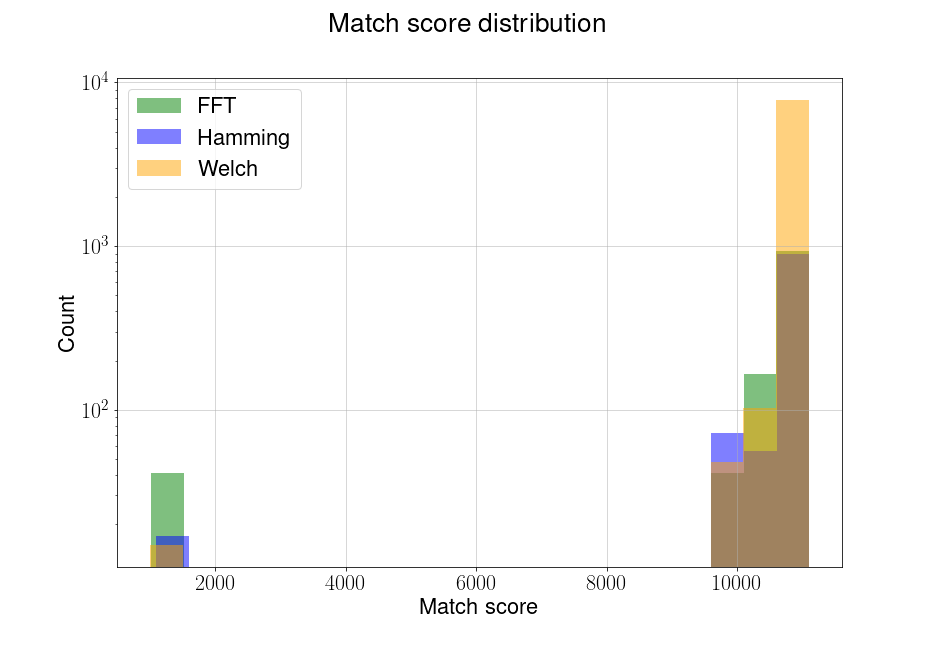
\includegraphics[width=.9\linewidth]{./img/match_score_dist.png}
\caption{\label{fig:orgbf258c1}Distribution of match scores}
\end{figure}

\section{Window Type}
\label{sec:org818d84e}
As shown in the in section \ref{org6276c12} the window type does play an important role in finding adequate results for the matching series.

Each window type can have side effects. As described in section \ref{orgeb5c515} windows help address the side effects of spectral leakage. However, the window can also lead to other effects. Consider a template series like in figure \ref{fig:orge9d512c} that has a particular dominant feature like the tooth shape visible in the template series. In the match that considers the median (d\textsubscript{q50}) as summary statistic we see an interesting result regarding Welch's method. Due to the fact that Welch's method slices the time series into multiple segments, applies a window and then averages the found frequencies one can see how a series that has the same dominant shape but multiple occurences of it produces a very similar result in the frequency domain. The median in this example must also have a similar value in both series as the ranges are similar. The second tooth in the pool series is just a repeption of the first, therefore the median is not affected significantly. And in consequence one receives a result that where a similar pattern repeats but the time series are still considered very similar.

When matching frequencies this will also include series that have the same pattern but multiple occurences of the pattern. Now if one chooses a summary statistic like minima, maxima or slopes one can find a result that has repetitions of this feature, and has them in different places compared to the template series.

\begin{figure}[htbp]
\centering
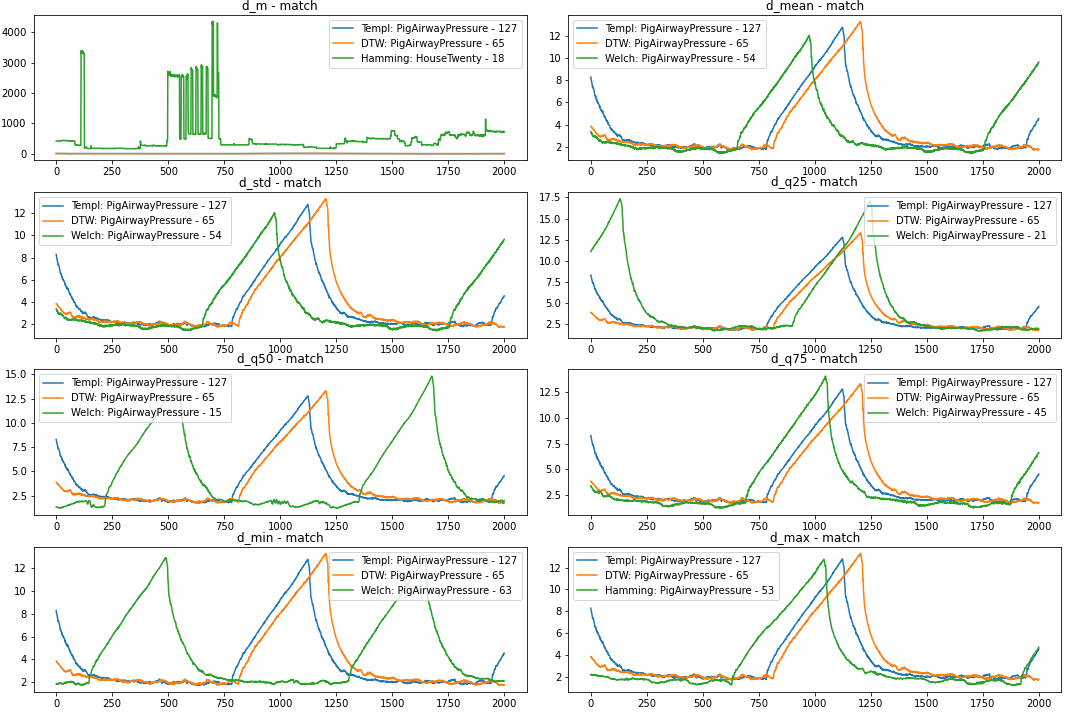
\includegraphics[width=.9\linewidth]{./img/dtw_comp_res/PigAirwayPressure_127.png}
\caption{\label{fig:orge9d512c}Repeating Pattern example - UCR: PigAirwayPressure - 127}
\end{figure}

Now whether the result is desirable depends on the context of the analysis or subsequent process the time series are to be utilized for. Therefore, it is expedient to work with different window types and summary statistics adequate for ones analytics requirement when searching for similar time series.

Some of the side-effects can be mitigated. For example with frequencies and chosen summary statistic may have a resulting time series from the pool that has a vastly different length compared to the template time series. This can be mitigated by imposing another restriction on the result set of the resulting series having to be within some treshold of length compared to the template. The DTW method mitigates this due to the fact that higher length series will lead to higher overall distance scores and hence will be ranked lower compared to shorter series whose points are also in a similar vicinity compared to the template series.

\section{Interesting examples}
\label{sec:orga29f063}
\ref{fig:org26ae65b} equally good result compared to DTW

Mixed result \ref{fig:orgfb1f273}


beautiful result \ref{fig:org4449995}
low frequency

\ref{fig:org0dd450a} - challenging task

\begin{itemize}
\item (maybe ) improvement in forecasting approach
\item find dataset with ground truth and compare DTW to this approach
\item Distance metrics
\item time complexity
\end{itemize}
\chapter{Conclusion \& future work}
\label{sec:org5651f95}

Due to the quality and the runtime of our algorithm it is feasible to use this method for real-time search engine that not only generates meaningful results of similar series but also allows flexibility in modifying the results in way that optimizes for particular statistical metrics. They can be chosen based on the subsequent data analysis or forecasting task at hand. Furthermore, some of the shortcomings of DTW are also are also addressed. Noise in the data is removed via the utilization of the top frequencies and the essence of each series pattern is captured.

Beneficial for the FFT-based algorithm is its scale-invariance. The Fourier domain is always reduced to the top k frequencies in the power spectrum, therefore the time compare two series is constant irrespective of the length. This advantage makes the analysis virtually independent of the time series length. This makes this application very interesting to fields where large quantities of time series need to be compared, like in financial analysis, or bio statistics, and others.

The frequency domain does not hold any information about the temporal domain. Therefore, it does not capture discernible information on trends, change points and the like. If those information are relevant to the time series comparison they need to be captured by the additional summary statistics. If computing such metrics is computationally expensive the overall effort in comparing the series increases. However, many scenarios can be covered with the simple and computationally cheap metrics covered in this thesis. This leads to another aspect that has to be carefully managed when utilizing the method proposed here. There is no single metric that guarantees good or even meaningful results. As the analytical requirements are different from task to task are different so are the metrics that are most helpful in identifying similar time series. This cannot be avoided by the steps presented here. Other methods, like Dynamic Time Warping provide such straightforward and easily rankable information. Again, whether those are applicable is a question of the analytical task at hand.

In its current implementation the time series similarity search algorithm produces inconsistent results. Some matches are spot on or resemble the results produced by DTW. Without reviewing the results from multiple statistics and window types a user may receive a time series that is not similar. Especially if a user requires quick or many results without wanting to review the each result manually a further improvement of the algorithm is required. We believe that finding a better way of reflecting the higher frequencies in the selection process without taking the middle frequencies to much into account will help solve this issue and produce more consistent results.


\section{Successes}
\label{sec:org5426584}
\section{Failures}
\label{sec:orgda645ab}
\section{Flaws}
\label{sec:org1cf00a9}
\begin{itemize}
\item final computation
\end{itemize}
\section{What is missing}
\label{sec:org7f0423b}
\begin{itemize}
\item denoising of time series
\item adjustment of number of frequencies used
\item 
\end{itemize}
\chapter{Results \& Discussion}
\label{sec:org547692c}
In this work we have shown that our proposed algorithm based on the Fast Fourier Transform (FFT) with frequency match scores augmented by summary statistics can be utilized to identify similar time series from a pool for a provided template works very fast compared to the standard method of Dynamic Time Warping (DTW) and creates very good overall results. Additionally we have applied multiple windows to the dataset to deal with the inherent short comings of the various techniques. The way of integrating the summary statistics gives a user the flexibility to adjust the algorithm to the needs of her specific anaytics task for which the similar time series are to be found.

The purpose of building a time series search engine can be achieved with this mechanism as results can be retrieved in sub seconds. This is a feat that would not be possible utilizing DTW for the same purpose.

The downside of utilizing our algorithm are that in its current form there are side effects which need to be considered, like retrieving series that have repeating patterns that do match in quantity or location depending on the used window type.

Future work, should focus on further enhancing the range association mechanism that better integrates the high frequency spectrum so that high frequencies are reflected accordingly in the identification 
\chapter{Visualizations of results}
\label{sec:org6db687d}
\label{orga341cff}
\begin{figure}[htbp]
\centering
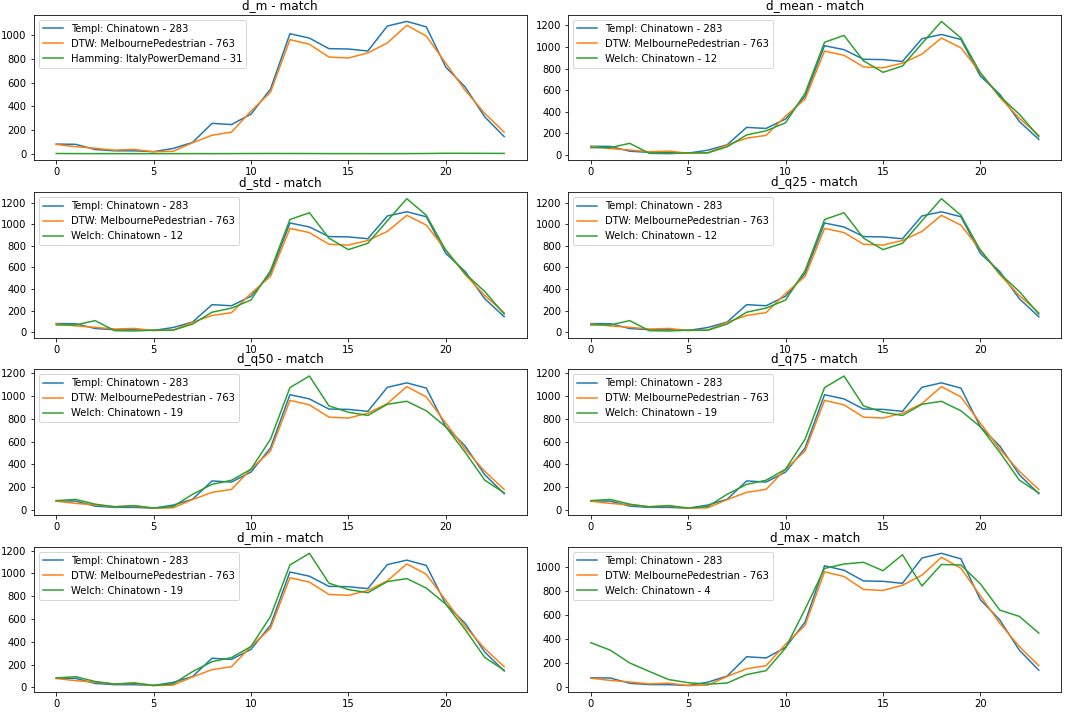
\includegraphics[width=.9\linewidth]{./img/dtw_comp_res/Chinatown_283.png}
\caption{\label{fig:org0c72bc6}Chinatown - 283}
\end{figure}

\begin{figure}[htbp]
\centering
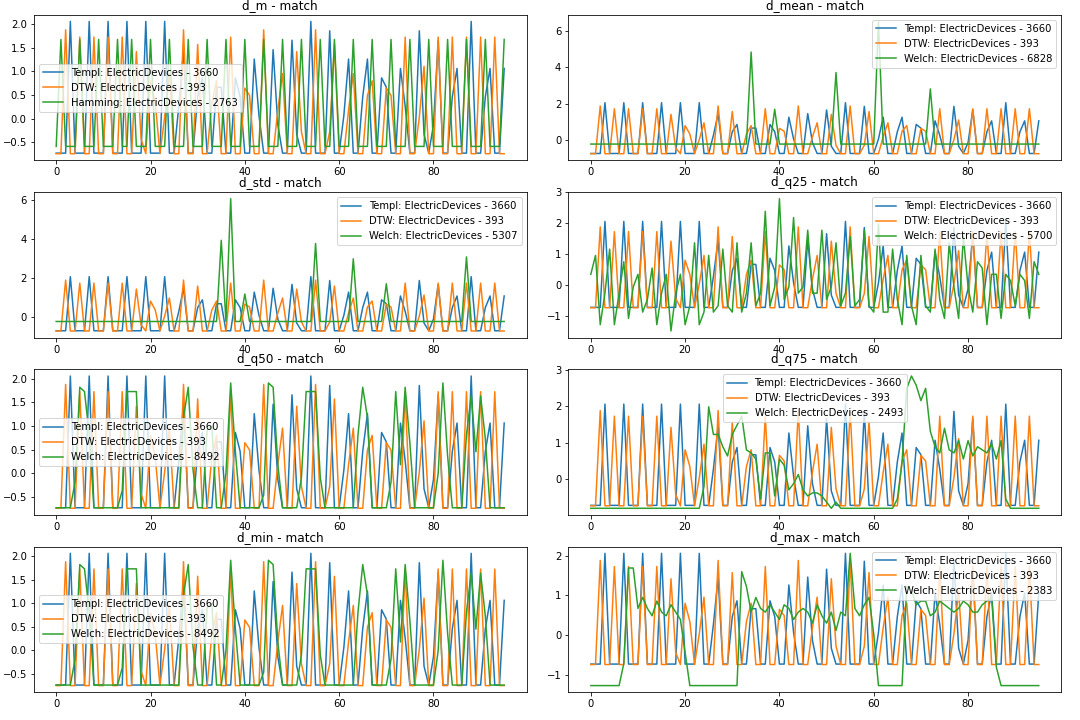
\includegraphics[width=.9\linewidth]{./img/dtw_comp_res/ElectricDevices_3660.png}
\caption{\label{fig:orgc85fd25}ElectricDevices - 3660}
\end{figure}

\begin{figure}[htbp]
\centering
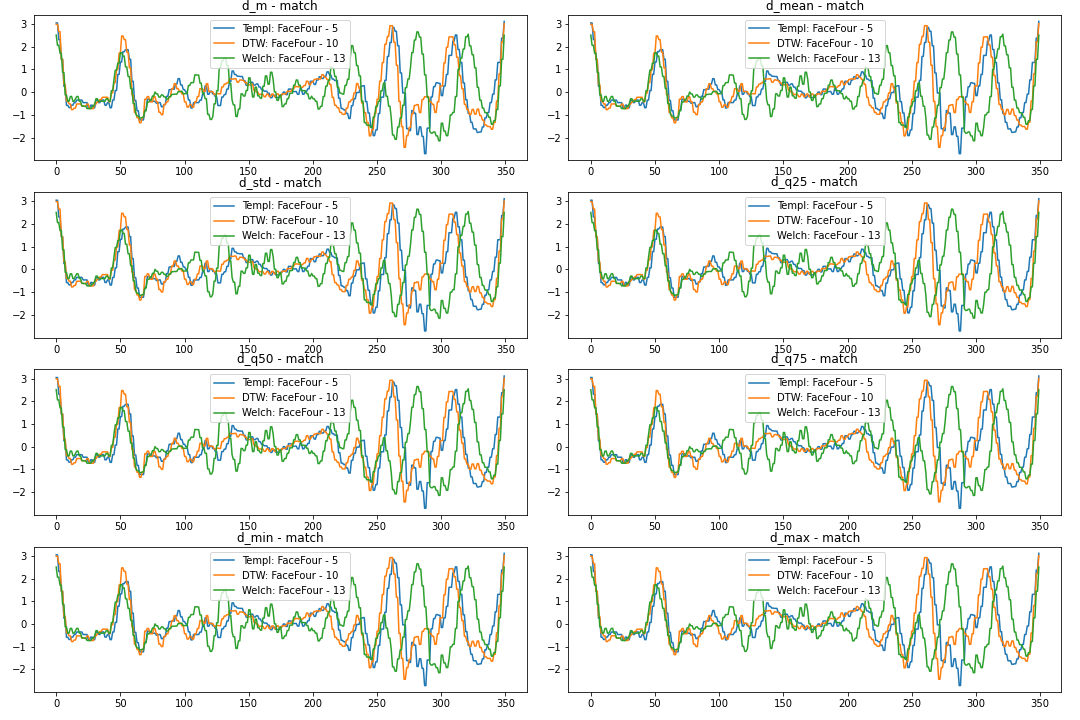
\includegraphics[width=.9\linewidth]{./img/dtw_comp_res/FaceFour_5.png}
\caption{\label{fig:org1a3bc56}FaceFour - 5}
\end{figure}

\begin{figure}[htbp]
\centering
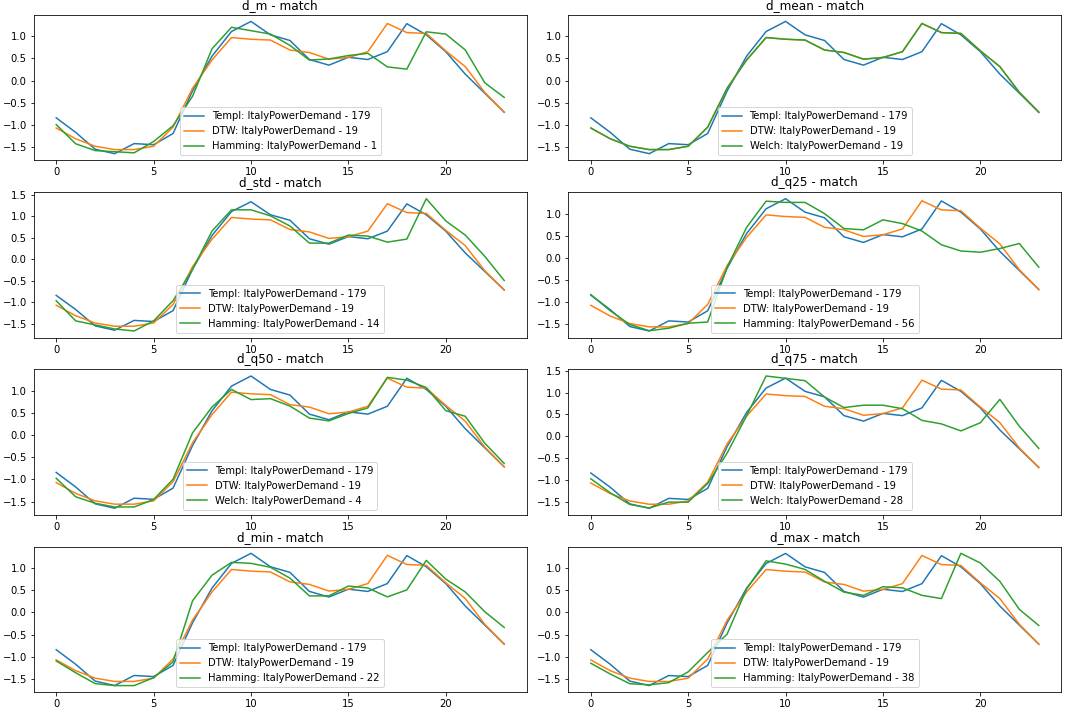
\includegraphics[width=.9\linewidth]{./img/dtw_comp_res/ItalyPowerDemand_179.png}
\caption{\label{fig:org26ae65b}ItalyPowerDemand - 179}
\end{figure}

\begin{figure}[htbp]
\centering
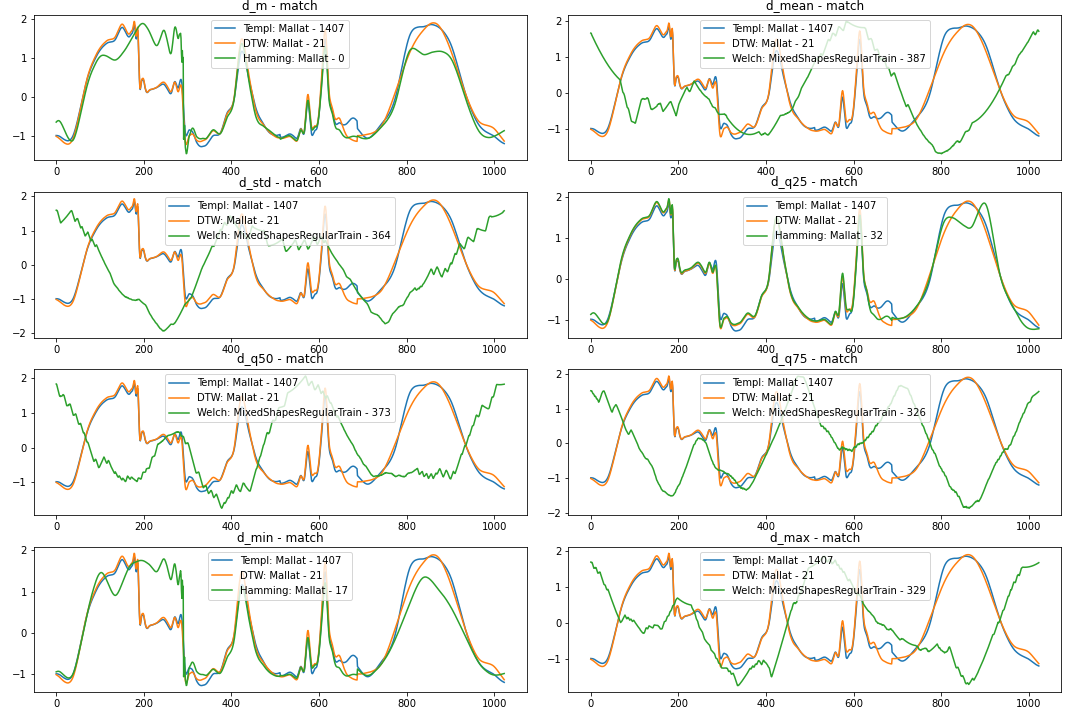
\includegraphics[width=.9\linewidth]{./img/dtw_comp_res/Mallat_1407.png}
\caption{\label{fig:orgfb1f273}Mallat - 1407}
\end{figure}

\begin{figure}[htbp]
\centering
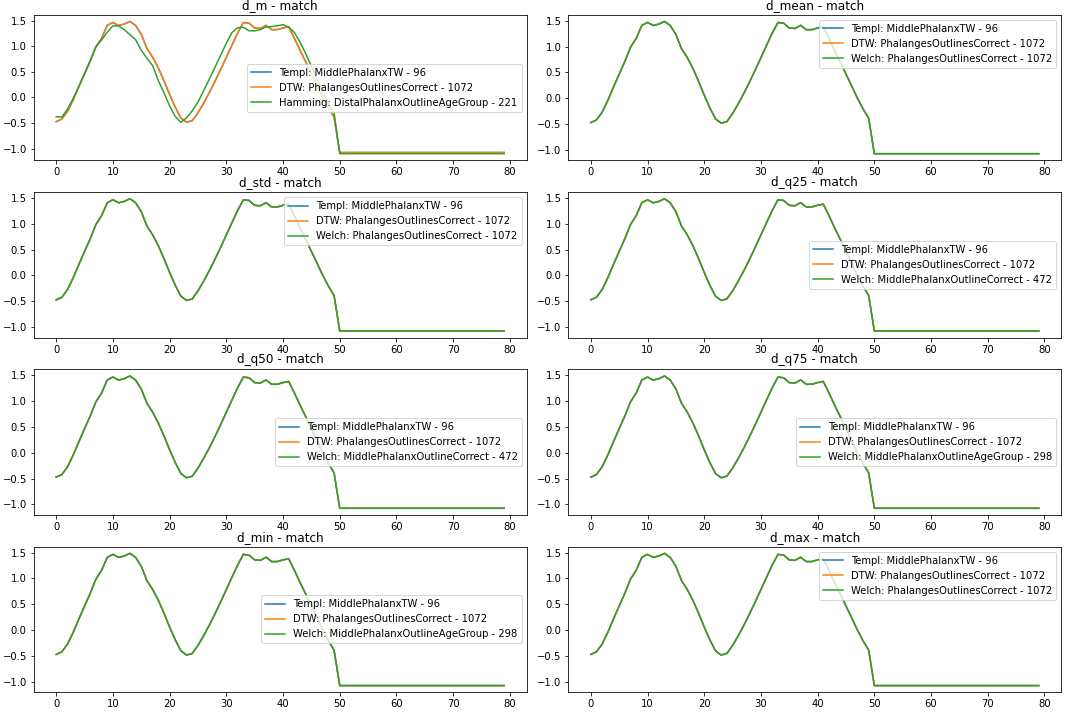
\includegraphics[width=.9\linewidth]{./img/dtw_comp_res/MiddlePhalanxTW_96.png}
\caption{\label{fig:org4449995}MiddlePhalanxTW - 96}
\end{figure}

\begin{figure}[htbp]
\centering
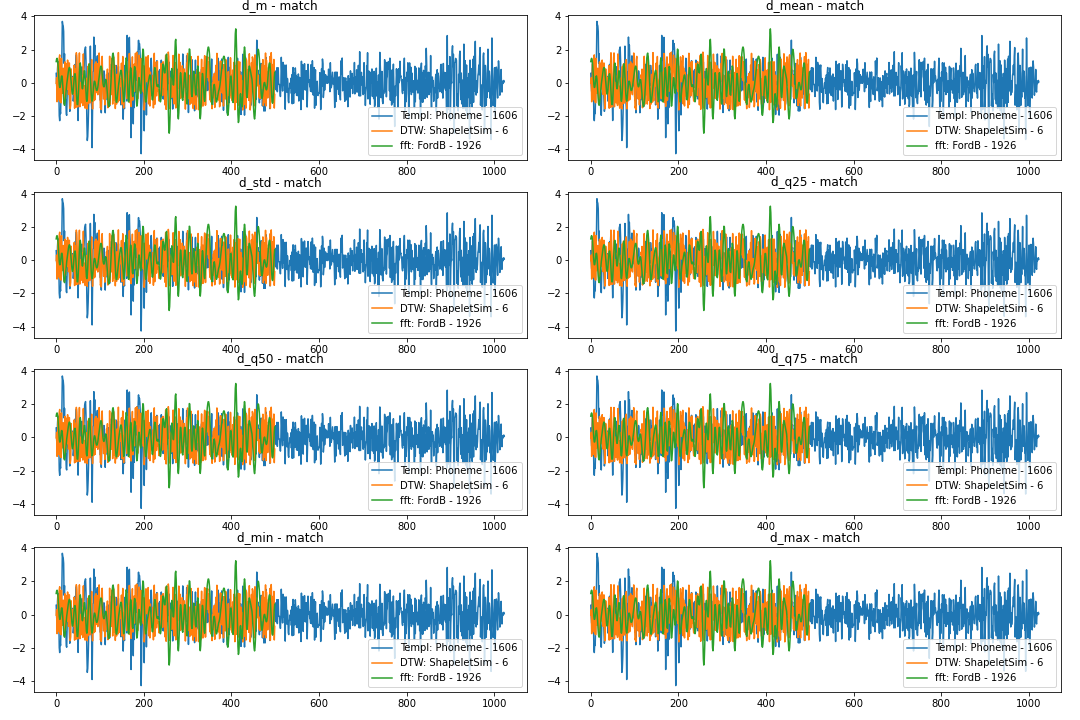
\includegraphics[width=.9\linewidth]{./img/dtw_comp_res/Phoneme_1606.png}
\caption{\label{fig:org0dd450a}Phoneme - 1606}
\end{figure}

\begin{figure}[htbp]
\centering
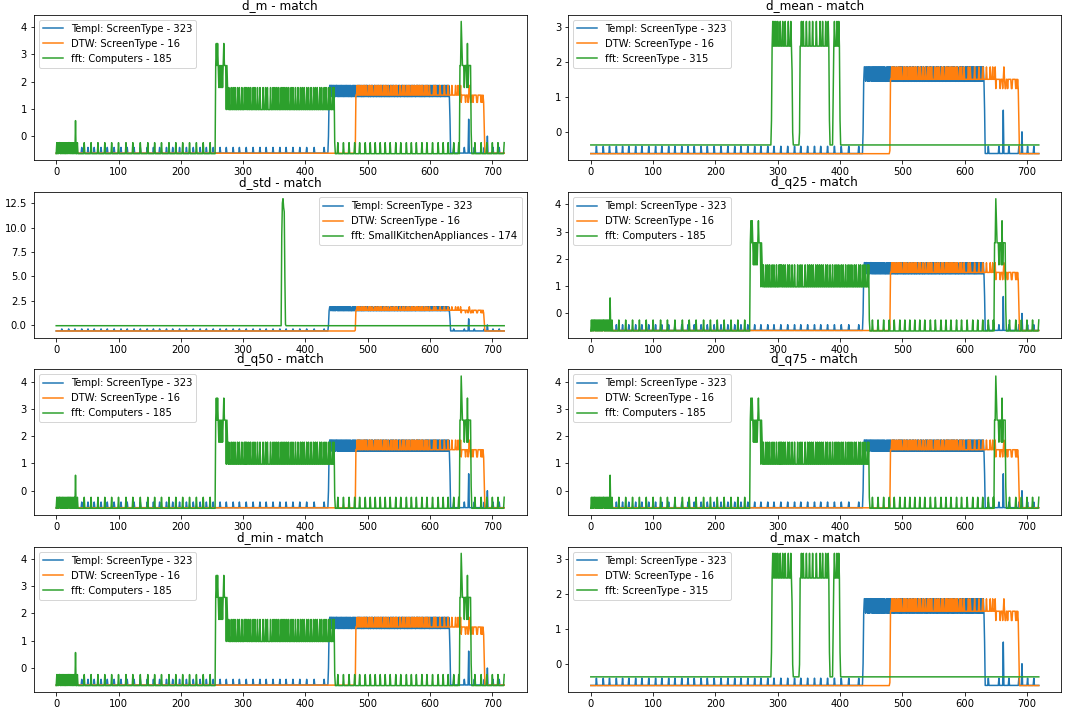
\includegraphics[width=.9\linewidth]{./img/dtw_comp_res/ScreenType_323.png}
\caption{\label{fig:org64009d8}ScreenType - 323}
\end{figure}

\begin{figure}[htbp]
\centering
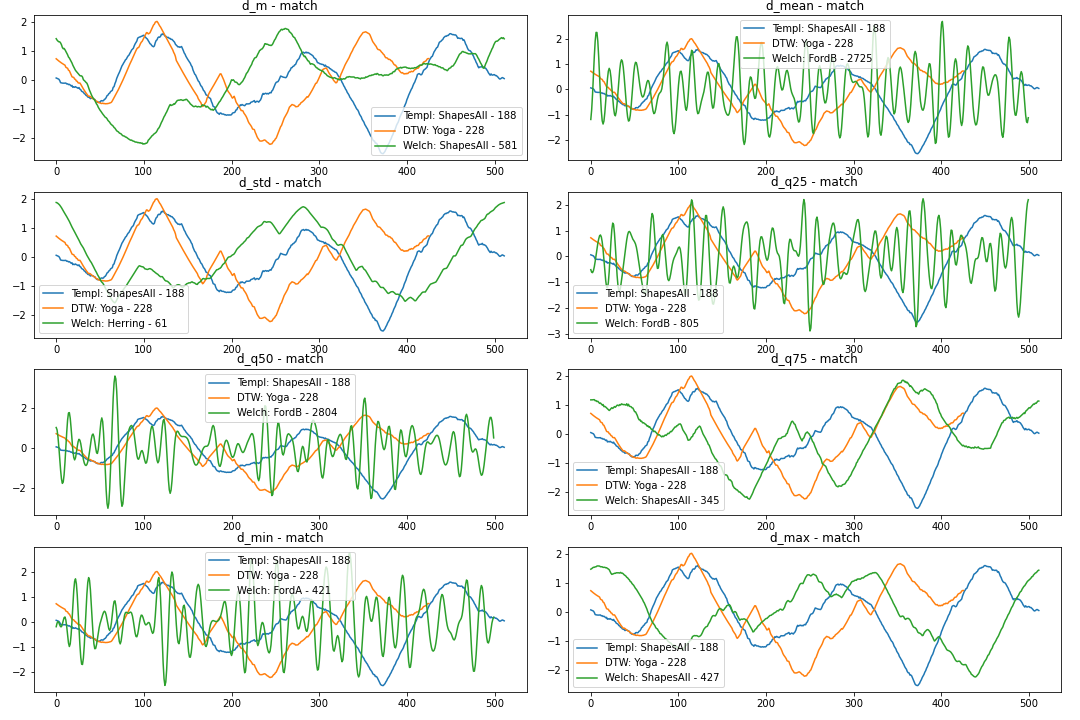
\includegraphics[width=.9\linewidth]{./img/dtw_comp_res/ShapesAll_188.png}
\caption{\label{fig:org54549bb}ShapesAll - 188}
\end{figure}

\begin{figure}[htbp]
\centering
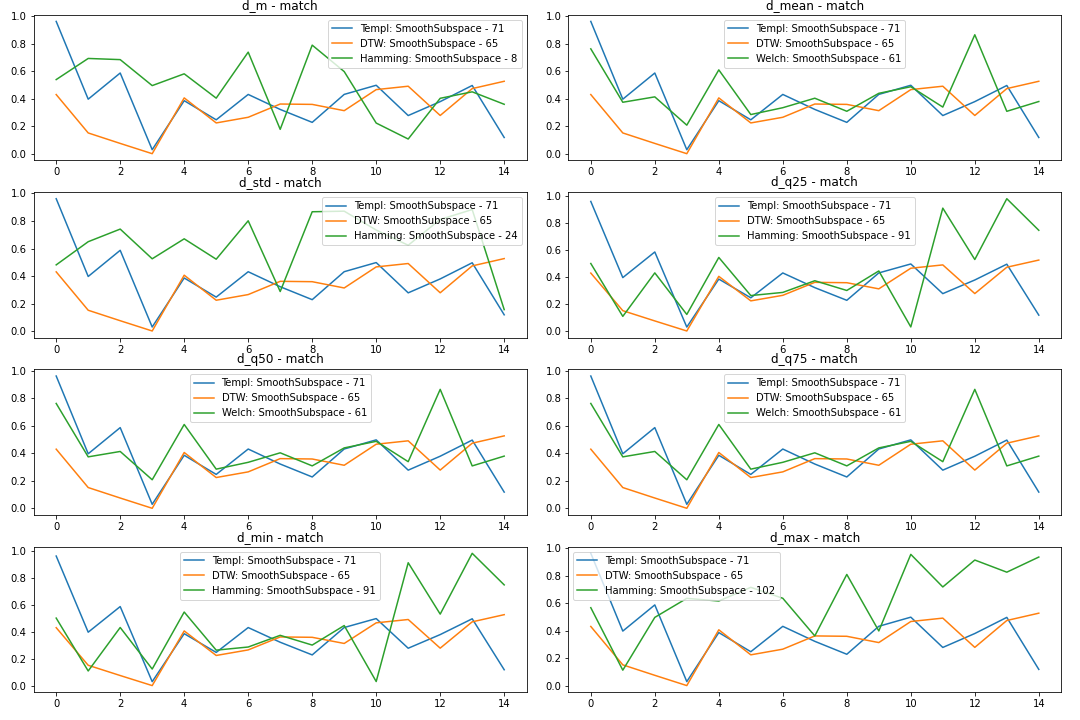
\includegraphics[width=.9\linewidth]{./img/dtw_comp_res/SmoothSubspace_71.png}
\caption{\label{fig:orgc2af2a3}SmoothSubspace - 71}
\end{figure}

\begin{figure}[htbp]
\centering
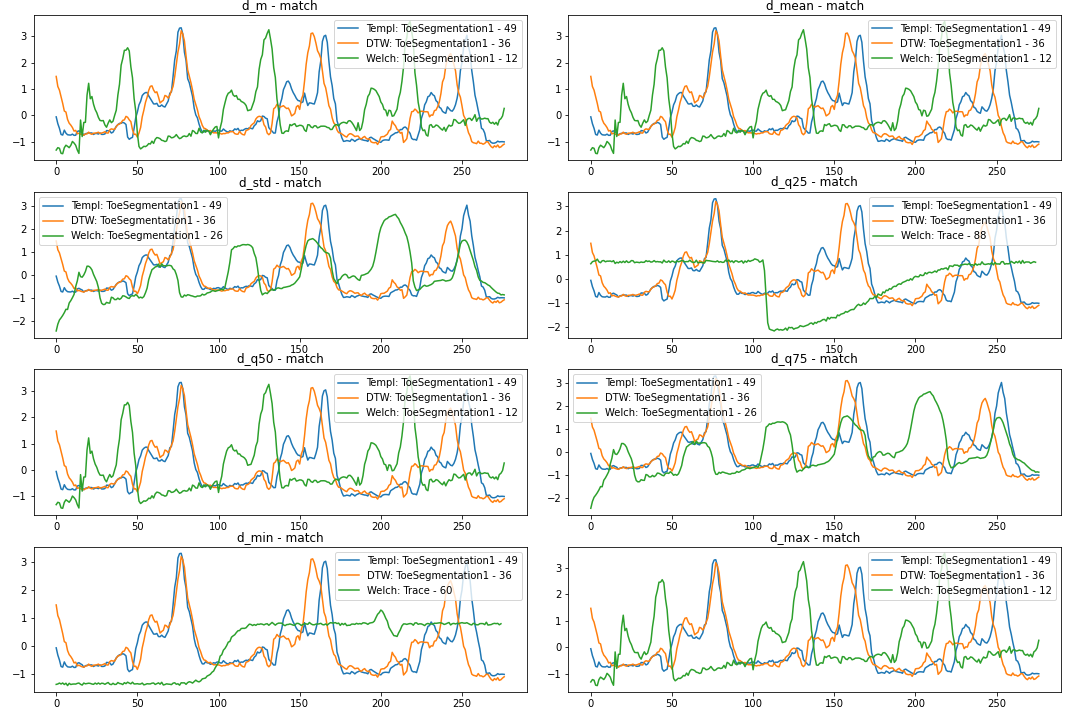
\includegraphics[width=.9\linewidth]{./img/dtw_comp_res/ToeSegmentation1_49.png}
\caption{\label{fig:orgd500ca2}ToeSegmentation1 - 49}
\end{figure}

\begin{figure}[htbp]
\centering
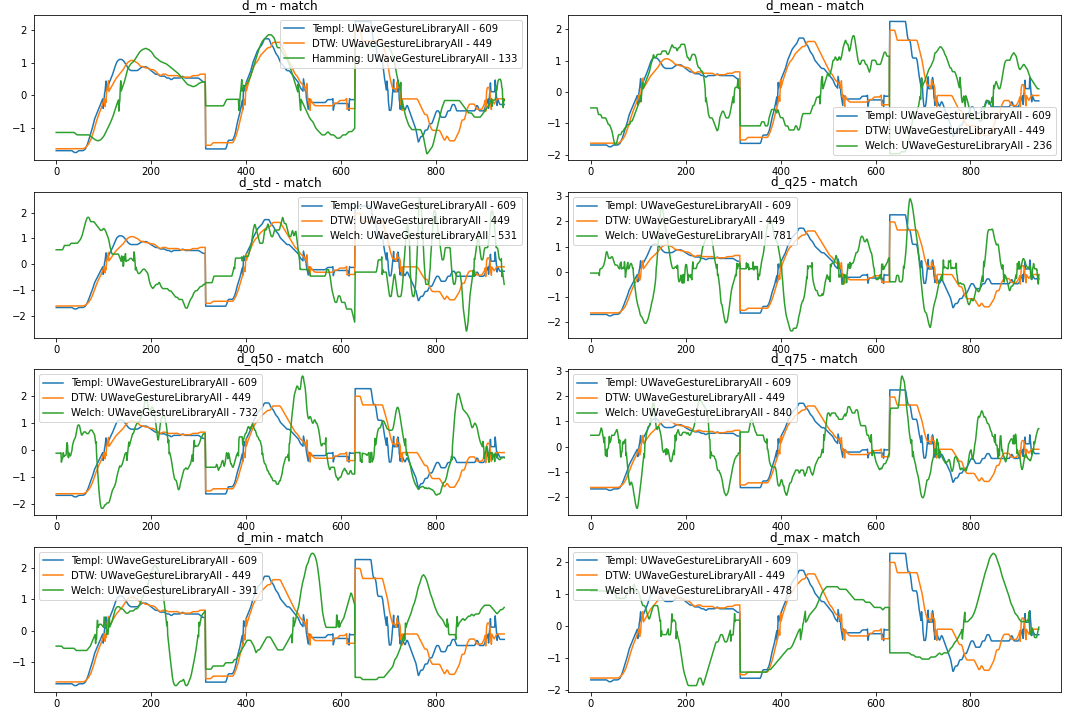
\includegraphics[width=.9\linewidth]{./img/dtw_comp_res/UWaveGestureLibraryAll_609.png}
\caption{\label{fig:orgec6077e}UWaveGestureLibraryAll - 609}
\end{figure}

\begin{figure}[htbp]
\centering
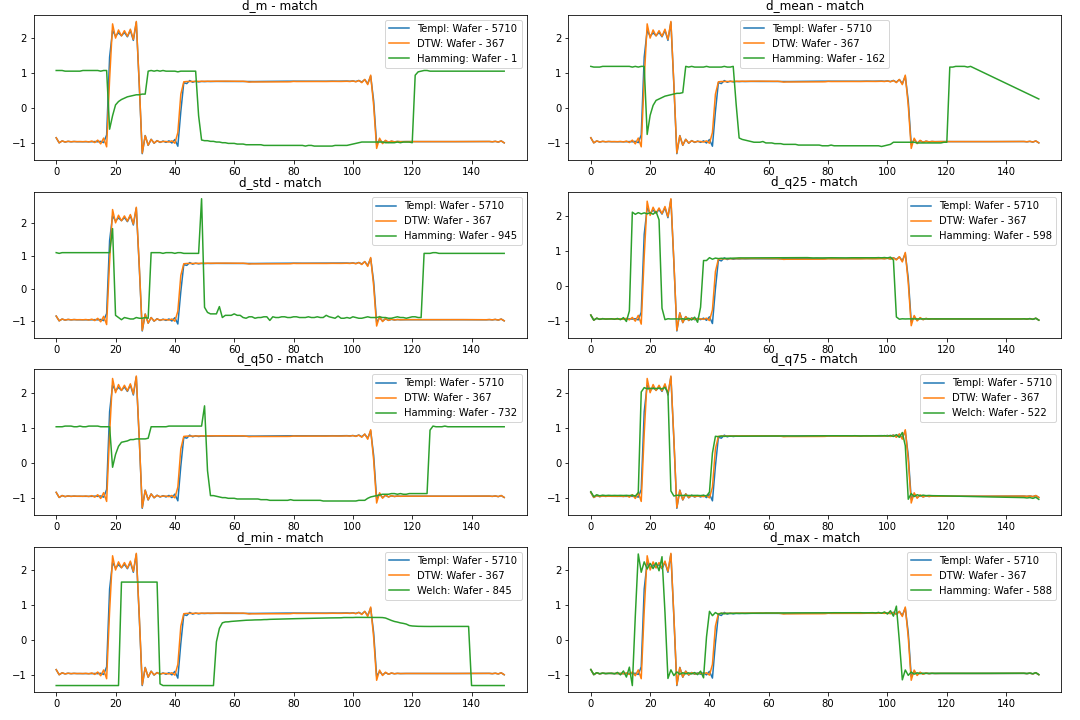
\includegraphics[width=.9\linewidth]{./img/dtw_comp_res/Wafer_5710.png}
\caption{\label{fig:orgbc531d0}Wafer - 5710}
\end{figure}

\bibliographystyle{abbrv}
\bibliography{thesis}
\end{document}